% Options for packages loaded elsewhere
\PassOptionsToPackage{unicode}{hyperref}
\PassOptionsToPackage{hyphens}{url}
\PassOptionsToPackage{dvipsnames,svgnames,x11names}{xcolor}
%
\documentclass[
  letterpaper,
  DIV=11,
  numbers=noendperiod]{scrartcl}

\usepackage{amsmath,amssymb}
\usepackage{iftex}
\ifPDFTeX
  \usepackage[T1]{fontenc}
  \usepackage[utf8]{inputenc}
  \usepackage{textcomp} % provide euro and other symbols
\else % if luatex or xetex
  \usepackage{unicode-math}
  \defaultfontfeatures{Scale=MatchLowercase}
  \defaultfontfeatures[\rmfamily]{Ligatures=TeX,Scale=1}
\fi
\usepackage{lmodern}
\ifPDFTeX\else  
    % xetex/luatex font selection
\fi
% Use upquote if available, for straight quotes in verbatim environments
\IfFileExists{upquote.sty}{\usepackage{upquote}}{}
\IfFileExists{microtype.sty}{% use microtype if available
  \usepackage[]{microtype}
  \UseMicrotypeSet[protrusion]{basicmath} % disable protrusion for tt fonts
}{}
\makeatletter
\@ifundefined{KOMAClassName}{% if non-KOMA class
  \IfFileExists{parskip.sty}{%
    \usepackage{parskip}
  }{% else
    \setlength{\parindent}{0pt}
    \setlength{\parskip}{6pt plus 2pt minus 1pt}}
}{% if KOMA class
  \KOMAoptions{parskip=half}}
\makeatother
\usepackage{xcolor}
\setlength{\emergencystretch}{3em} % prevent overfull lines
\setcounter{secnumdepth}{5}
% Make \paragraph and \subparagraph free-standing
\makeatletter
\ifx\paragraph\undefined\else
  \let\oldparagraph\paragraph
  \renewcommand{\paragraph}{
    \@ifstar
      \xxxParagraphStar
      \xxxParagraphNoStar
  }
  \newcommand{\xxxParagraphStar}[1]{\oldparagraph*{#1}\mbox{}}
  \newcommand{\xxxParagraphNoStar}[1]{\oldparagraph{#1}\mbox{}}
\fi
\ifx\subparagraph\undefined\else
  \let\oldsubparagraph\subparagraph
  \renewcommand{\subparagraph}{
    \@ifstar
      \xxxSubParagraphStar
      \xxxSubParagraphNoStar
  }
  \newcommand{\xxxSubParagraphStar}[1]{\oldsubparagraph*{#1}\mbox{}}
  \newcommand{\xxxSubParagraphNoStar}[1]{\oldsubparagraph{#1}\mbox{}}
\fi
\makeatother

\usepackage{color}
\usepackage{fancyvrb}
\newcommand{\VerbBar}{|}
\newcommand{\VERB}{\Verb[commandchars=\\\{\}]}
\DefineVerbatimEnvironment{Highlighting}{Verbatim}{commandchars=\\\{\}}
% Add ',fontsize=\small' for more characters per line
\usepackage{framed}
\definecolor{shadecolor}{RGB}{241,243,245}
\newenvironment{Shaded}{\begin{snugshade}}{\end{snugshade}}
\newcommand{\AlertTok}[1]{\textcolor[rgb]{0.68,0.00,0.00}{#1}}
\newcommand{\AnnotationTok}[1]{\textcolor[rgb]{0.37,0.37,0.37}{#1}}
\newcommand{\AttributeTok}[1]{\textcolor[rgb]{0.40,0.45,0.13}{#1}}
\newcommand{\BaseNTok}[1]{\textcolor[rgb]{0.68,0.00,0.00}{#1}}
\newcommand{\BuiltInTok}[1]{\textcolor[rgb]{0.00,0.23,0.31}{#1}}
\newcommand{\CharTok}[1]{\textcolor[rgb]{0.13,0.47,0.30}{#1}}
\newcommand{\CommentTok}[1]{\textcolor[rgb]{0.37,0.37,0.37}{#1}}
\newcommand{\CommentVarTok}[1]{\textcolor[rgb]{0.37,0.37,0.37}{\textit{#1}}}
\newcommand{\ConstantTok}[1]{\textcolor[rgb]{0.56,0.35,0.01}{#1}}
\newcommand{\ControlFlowTok}[1]{\textcolor[rgb]{0.00,0.23,0.31}{\textbf{#1}}}
\newcommand{\DataTypeTok}[1]{\textcolor[rgb]{0.68,0.00,0.00}{#1}}
\newcommand{\DecValTok}[1]{\textcolor[rgb]{0.68,0.00,0.00}{#1}}
\newcommand{\DocumentationTok}[1]{\textcolor[rgb]{0.37,0.37,0.37}{\textit{#1}}}
\newcommand{\ErrorTok}[1]{\textcolor[rgb]{0.68,0.00,0.00}{#1}}
\newcommand{\ExtensionTok}[1]{\textcolor[rgb]{0.00,0.23,0.31}{#1}}
\newcommand{\FloatTok}[1]{\textcolor[rgb]{0.68,0.00,0.00}{#1}}
\newcommand{\FunctionTok}[1]{\textcolor[rgb]{0.28,0.35,0.67}{#1}}
\newcommand{\ImportTok}[1]{\textcolor[rgb]{0.00,0.46,0.62}{#1}}
\newcommand{\InformationTok}[1]{\textcolor[rgb]{0.37,0.37,0.37}{#1}}
\newcommand{\KeywordTok}[1]{\textcolor[rgb]{0.00,0.23,0.31}{\textbf{#1}}}
\newcommand{\NormalTok}[1]{\textcolor[rgb]{0.00,0.23,0.31}{#1}}
\newcommand{\OperatorTok}[1]{\textcolor[rgb]{0.37,0.37,0.37}{#1}}
\newcommand{\OtherTok}[1]{\textcolor[rgb]{0.00,0.23,0.31}{#1}}
\newcommand{\PreprocessorTok}[1]{\textcolor[rgb]{0.68,0.00,0.00}{#1}}
\newcommand{\RegionMarkerTok}[1]{\textcolor[rgb]{0.00,0.23,0.31}{#1}}
\newcommand{\SpecialCharTok}[1]{\textcolor[rgb]{0.37,0.37,0.37}{#1}}
\newcommand{\SpecialStringTok}[1]{\textcolor[rgb]{0.13,0.47,0.30}{#1}}
\newcommand{\StringTok}[1]{\textcolor[rgb]{0.13,0.47,0.30}{#1}}
\newcommand{\VariableTok}[1]{\textcolor[rgb]{0.07,0.07,0.07}{#1}}
\newcommand{\VerbatimStringTok}[1]{\textcolor[rgb]{0.13,0.47,0.30}{#1}}
\newcommand{\WarningTok}[1]{\textcolor[rgb]{0.37,0.37,0.37}{\textit{#1}}}

\providecommand{\tightlist}{%
  \setlength{\itemsep}{0pt}\setlength{\parskip}{0pt}}\usepackage{longtable,booktabs,array}
\usepackage{calc} % for calculating minipage widths
% Correct order of tables after \paragraph or \subparagraph
\usepackage{etoolbox}
\makeatletter
\patchcmd\longtable{\par}{\if@noskipsec\mbox{}\fi\par}{}{}
\makeatother
% Allow footnotes in longtable head/foot
\IfFileExists{footnotehyper.sty}{\usepackage{footnotehyper}}{\usepackage{footnote}}
\makesavenoteenv{longtable}
\usepackage{graphicx}
\makeatletter
\def\maxwidth{\ifdim\Gin@nat@width>\linewidth\linewidth\else\Gin@nat@width\fi}
\def\maxheight{\ifdim\Gin@nat@height>\textheight\textheight\else\Gin@nat@height\fi}
\makeatother
% Scale images if necessary, so that they will not overflow the page
% margins by default, and it is still possible to overwrite the defaults
% using explicit options in \includegraphics[width, height, ...]{}
\setkeys{Gin}{width=\maxwidth,height=\maxheight,keepaspectratio}
% Set default figure placement to htbp
\makeatletter
\def\fps@figure{htbp}
\makeatother

\KOMAoption{captions}{tableheading}
\makeatletter
\@ifpackageloaded{caption}{}{\usepackage{caption}}
\AtBeginDocument{%
\ifdefined\contentsname
  \renewcommand*\contentsname{Table of contents}
\else
  \newcommand\contentsname{Table of contents}
\fi
\ifdefined\listfigurename
  \renewcommand*\listfigurename{List of Figures}
\else
  \newcommand\listfigurename{List of Figures}
\fi
\ifdefined\listtablename
  \renewcommand*\listtablename{List of Tables}
\else
  \newcommand\listtablename{List of Tables}
\fi
\ifdefined\figurename
  \renewcommand*\figurename{Figure}
\else
  \newcommand\figurename{Figure}
\fi
\ifdefined\tablename
  \renewcommand*\tablename{Table}
\else
  \newcommand\tablename{Table}
\fi
}
\@ifpackageloaded{float}{}{\usepackage{float}}
\floatstyle{ruled}
\@ifundefined{c@chapter}{\newfloat{codelisting}{h}{lop}}{\newfloat{codelisting}{h}{lop}[chapter]}
\floatname{codelisting}{Listing}
\newcommand*\listoflistings{\listof{codelisting}{List of Listings}}
\makeatother
\makeatletter
\makeatother
\makeatletter
\@ifpackageloaded{caption}{}{\usepackage{caption}}
\@ifpackageloaded{subcaption}{}{\usepackage{subcaption}}
\makeatother

\ifLuaTeX
  \usepackage{selnolig}  % disable illegal ligatures
\fi
\usepackage{bookmark}

\IfFileExists{xurl.sty}{\usepackage{xurl}}{} % add URL line breaks if available
\urlstyle{same} % disable monospaced font for URLs
\hypersetup{
  pdftitle={DATA3888: Predicting Stock Volatility},
  pdfauthor={Ayush Singh, Tobit Louis, Kylie Haryono, Christy Lee, Zichun Han},
  colorlinks=true,
  linkcolor={blue},
  filecolor={Maroon},
  citecolor={Blue},
  urlcolor={Blue},
  pdfcreator={LaTeX via pandoc}}


\title{DATA3888: Predicting Stock Volatility}
\author{Ayush Singh, Tobit Louis, Kylie Haryono, Christy Lee, Zichun
Han}
\date{2025-05-24}

\begin{document}
\maketitle

\renewcommand*\contentsname{Table of contents}
{
\hypersetup{linkcolor=}
\setcounter{tocdepth}{3}
\tableofcontents
}

\section{Executive Summary}\label{executive-summary}

\subsection{Research Question}\label{research-question}

Short-term volatility forecasting is critical for high-frequency
trading, risk management, and market-making. This study investigates
whether advanced deep learning architectures can enhance predictive
accuracy using ultra-high-frequency Level-2 Limit Order Book (LOB) data.
Specifically, we evaluate whether a Transformer-based model can
outperform traditional Long Short-Term Memory (LSTM) networks when both
models are trained on identically preprocessed datasets with equivalent
engineered features. The goal is to determine if the Transformer's
attention mechanism offers a material advantage in capturing complex
microstructural dynamics inherent in LOB data.

\subsubsection{Hypothesis}\label{hypothesis}

\paragraph{Null Hypothesis (H₀)}\label{null-hypothesis-hux2080}

Given equivalent data quality, feature engineering, and preprocessing
conditions, a Transformer-based model does not outperform LSTM networks
in short-term volatility forecasting on Level-2 Limit Order Book (LOB)
data.

\paragraph{Alternative Hypothesis
(H₁)}\label{alternative-hypothesis-hux2081}

Given equivalent data quality, feature engineering, and preprocessing
conditions, a Transformer-based model outperforms LSTM networks in
short-term volatility forecasting on Level-2 Limit Order Book (LOB)
data.

\subsection{Key Findings}\label{key-findings}

Our analysis shows that the Transformer model achieves superior
performance in short-term volatility forecasting, consistently
outperforming over 15 candidate models. In general, it attains an
\textbf{out-of-sample R² of 0.62} and \textbf{QLIKE loss of 0.14},
capturing 62\% of realized volatility variation---substantially higher
than the WLS and Random Forest baselines, and measurably better than the
LSTM. In favorable market regimes, performance improves to
\textbf{out-of-sample R² of 0.78} and \textbf{QLIKE loss of 0.05}. The
Transformer's attention mechanism effectively identifies temporally
localized predictive structures in high-frequency order flow, yielding
robust and highly accurate forecasts.

\begin{figure}[H]

{\centering 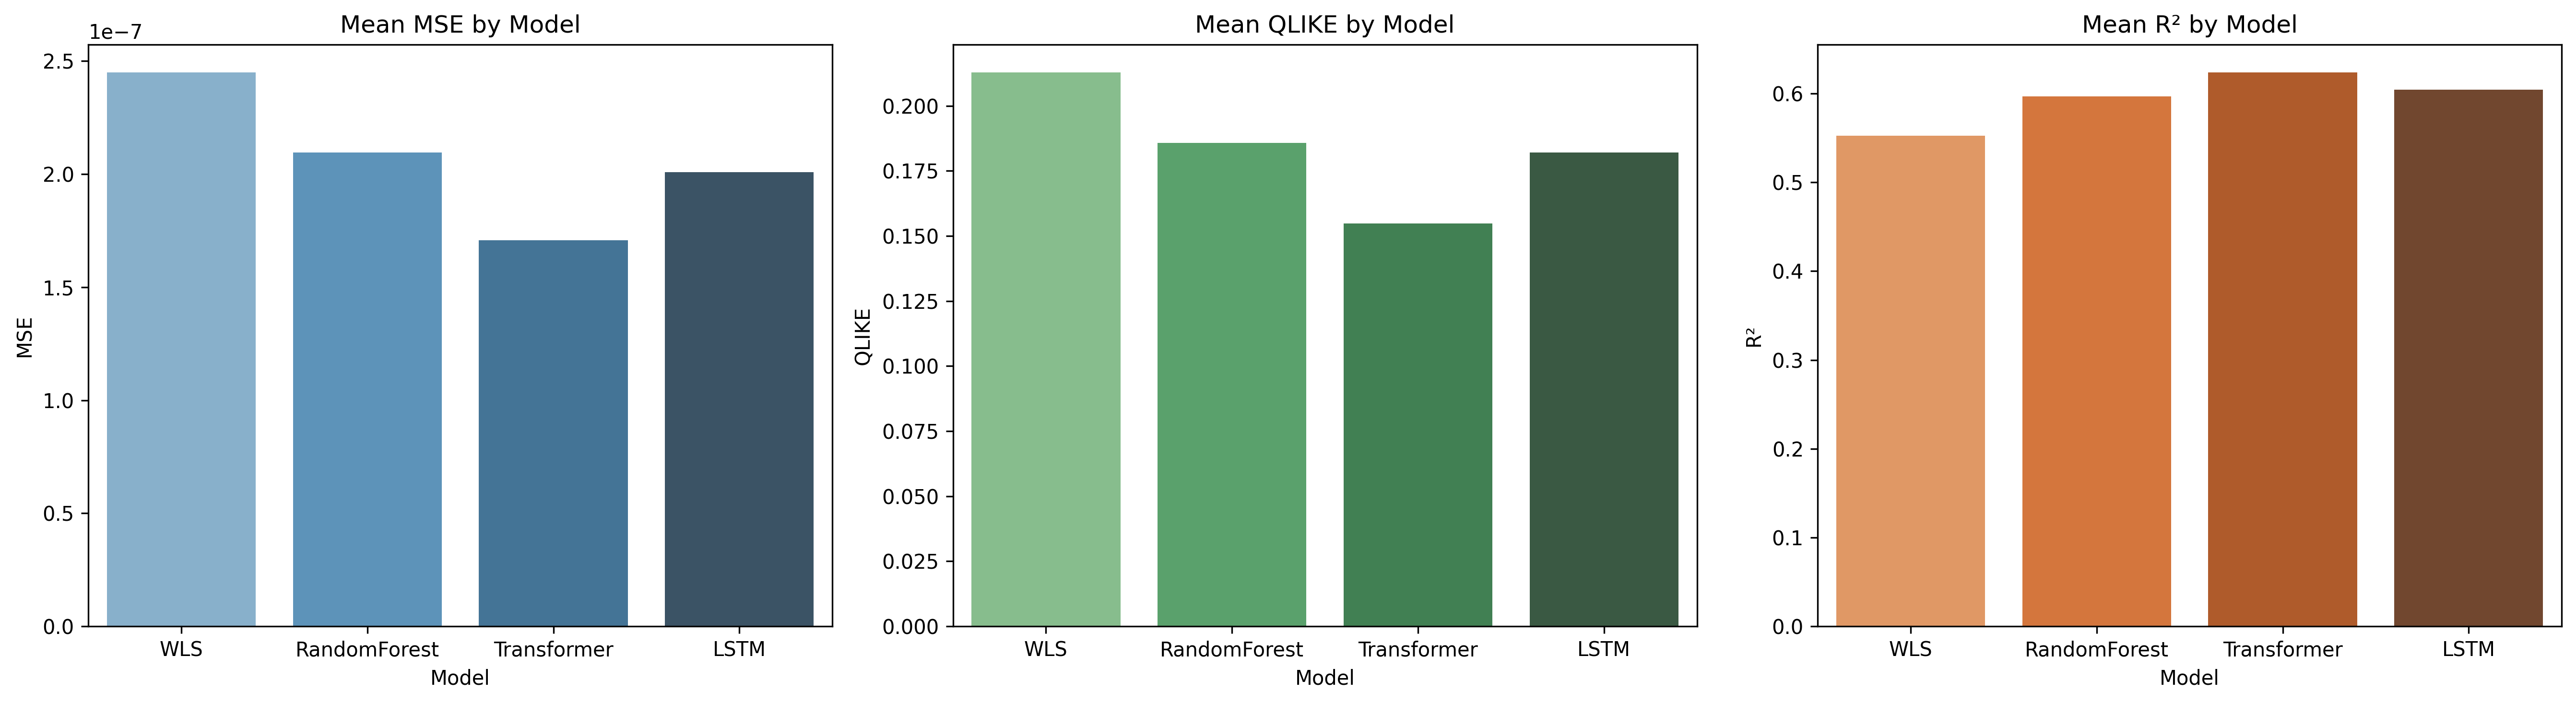
\includegraphics[width=1\textwidth,height=\textheight]{model_comparison.png}

}

\caption{Bar plots of Mean MSE, QLIKE, and R² by Model}

\end{figure}%

\subsection{Relevance}\label{relevance}

The demonstrated predictive accuracy of the Transformer model has direct
implications for high-frequency trading, risk management, and option
pricing. High-quality real-time volatility estimates support tighter
bid-ask spreads, more efficient hedging, and improved capital deployment
under microsecond constraints. By capturing core properties of
stochastic volatility---namely clustering, persistence, and
asymmetry---the Transformer enables materially better real-time
decision-making in trading and portfolio optimization contexts.

\section{EDA}\label{eda}

The Exploratory Data Analysis (EDA) stage involves data quality
assessment and feature engineering, which were key to processing the
dataset for time-series modelling. High frequency financial data may
present challenges such as irregular sampling, missing observations, and
noise that must be first addressed.

Considering the consecutive nature of the time series data, it is
essential to keep missing data to a minimum and dealing with it
systematically. Time IDs with at least 70\% missing seconds are taken
out of the used dataset. Bar charts were also used to visualise the
distribution of missing percentages across time buckets, missing seconds
in bucket per time ID, and missing seconds across time buckets.

Little's Missing Completely At Random (MCAR) Test was applied to check
for patterns in missing data, and consequently whether imputation was
appropriate. The result showed a high p-value of 1.00, indicating that
the missing data is indeed MCAR and not dependent on other variables. We
followed up by imputing low missing time intervals along with removing
high missing time intervals to maintain the integrity of the dataset and
utilising all available data that is reliable.

\subsection{Feature Engineering}\label{feature-engineering}

During the pre-cleaning stage, corrupt or out-of-range LOB records are
removed. This includes (1) non-positive prices and sizes, (2) crossed
quotes (ask \textless{} bid) at both levels, (3) seconds\_in\_bucket
outside of the expected range, and (4) duplicate or non-monotonic
timestamps within each time\_id. For the train-test split, 70-30 split
was used, non-randomised to keep the consecutive nature of the data.
After aggregating the features, the dataset is winsorised to reduce the
impact of outliers. This scaling method is done by replacing the extreme
values with less extreme values from the dataset.

The feature selection process uses two criteria: Pearson Correlation and
Mutual Information. Pearson correlation and mutual information are
calculated between each feature and the target variable, with Pearson
correlation measuring linear relationships between the variables while
mutual information captures the non-linear aspects. The features are
then selected if it meets either of two criteria: it has absolute
Pearson correlation of higher than or equal to 0.10, or mutual
information score higher or equal to 75th percentile.

\subsection{Testing}\label{testing}

In establishing a baseline, the naive prediction was made using the
current realised volatility. It calculates the Root Mean Squared Error
(RMSE) of this baseline, which was 0.92. This represents how well you
would do by simply assuming tomorrow's volatility is the same as
today's.

There were several regression models trained and evaluated in the
process. Ridge Regression had a test RMSE of 0.56, while Random Forest
had a test RMSE of 0.55, and LightGBM and Histogram-based Gradient
Boosting both had test RMSEs of 0.50 each. The decreasing RMSE values
show increasingly better performance. The gradient boosting models
(LightGBM and Histogram GBM) both had the best performance, reducing the
prediction error by approximately 46\% from the naive approach. This
suggests that the features selected contain valuable predictive
information about future volatility, and that tree-based ensembles
performed better at capturing complex relationships in this data than
linear models like Ridge Regression.

\section{Model Selection}\label{model-selection}

After developing over 15 models, we strategically selected the following
four models for detailed analysis including two top-performing
models---Transformer and LSTM, along with a baseline model demonstrating
solid foundational performance -- Weighted Least Squares (WLS), and a
high-performing model within its complexity class -- Random Forest,
which consistently outperformed other models of comparable complexity.

Our first implementation was a lightweight Transformer encoder for
volatility forecasting. This involved projecting each 30 step LOB
sequence into a 64-dimensional embedding, then stacking two encoder
blocks---each with four-head self-attention with a key/query dimension
of 64, a 4× feed-forward expansion to 256 units, and both
residual and layer-norm connections. After global average pooling, a
single linear output head produces the forecast, totaling an estimate of
100, 000 parameters. Inputs and log-transformed targets were
MinMax-scaled. Training used the Adam optimiser with a learning rate of
1 × 10⁻³, using Mean Squared Error (MSE) loss on a strict 80/10/10
chronological split, a batch size of 32, and early stopping with a
patience of 15 over 50 epochs. The model required approximately 500
GPU-hours to train and delivered strong out-of-sample RMSE, R², and
QLIKE performance.

For our next model, we built a two-layer stacked LSTM. with 64 units
returning all 30 steps (\textasciitilde25 088 parameters), followed by
20 \% dropout, then a 32-unit LSTM (\textasciitilde12 416 parameters)
with another 20 \% dropout---topped by a compact feed-forward head
(16-node dense + single linear output, \textasciitilde545 parameters),
for \textasciitilde38 k trainable weights. Inputs were min-max--scaled
30-step sequences of engineered LOB features and the target was
log-transformed volatility. We enforced a strict chronological split (80
\% train, 10 \% val, 10 \% test) to eliminate look-ahead bias, trained
with Adam at a 1 × 10⁻⁴ learning rate, 128-sample batches, and early
stopping (patience = 5) for up to 50 epochs. Out-of-sample RMSE, R², and
QLIKE metrics demonstrate strong sequence learning and stable volatility
forecasts.

For the next model, a two-layer stacked LSTM was built. The first layer
consisted of 64 units returning all 30 steps, comprising approximately
25,088 parameters, followed by 20\% dropout. This was then followed by a
32-unit LSTM layer with around 12,416 parameters and another 20\%
dropout. This architecture was topped by a compact feed-forward head,
consisting of a 16-node dense layer and a single linear output,
contributing approximately 545 parameters, for a total of approximately
38,000 trainable weights. Inputs were MinMax-scaled 30-step sequences of
engineered LOB features, and the target was log-transformed volatility.
A strict chronological split of 80\% for training, 10\% for validation,
and 10\% for testing was enforced to eliminate look-ahead bias. Training
was conducted using the Adam optimizer with a 1×10−4 learning rate,
128-sample batches, and early stopping with a patience of 5 for up to 50
epochs. Out-of-sample RMSE, R², and QLIKE metrics demonstrated strong
sequence learning and stable volatility forecasts.

Next, we used an ensemble of 500 trees grown to full depth, sampling the
square root of features at each split and enforcing a minimum of three
samples per leaf. Bootstrap aggregation was used to decorrelate trees
and reduce variance. The volatility target was log-transformed to
stabilize its heavy-tailed distribution, and we partitioned the data
chronologically---80\% for training, 10\% for validation, 10\% for
testing---to eliminate look-ahead bias. Training ran in parallel across
all CPU cores for efficiency, and we monitored progress in real time.
Out-of-sample performance was measured with root-mean-square error and
QLIKE loss (with clipping), demonstrating the model's ability to capture
complex nonlinear interactions in order-book dynamics.

Finally, we implemented a heteroskedasticity-aware WLS model in
statsmodels to forecast 30-tick-ahead realized volatility. Observation
weights were set as the inverse of a long-window rolling variance to
counter time-varying noise. Using a chronological 80/20 train-test split
across all 30 stocks, the model delivers a strong baseline out-of-sample
R² and QLIKE loss.

\section{Model Evaluation}\label{model-evaluation}

\subsection{Metrics Used}\label{metrics-used}

To evaluate model performance comprehensively, we used three
complementary metrics:

\begin{itemize}
\item
  \textbf{R-squared (R²)}: This measures how much of the variance in the
  target variable is explained by the model. A higher R² means the
  model's predictions align more closely with actual volatility, giving
  a good sense of overall fit.
\item
  \textbf{QLIKE (Quasi-Likelihood) Loss}: Tailored for volatility
  forecasting, QLIKE penalises underestimates more heavily than
  overestimates. This is especially important in financial risk
  settings, where underpredicting volatility can lead to poor hedging or
  mispricing.
\item
  \textbf{Mean Squared Error (MSE)}: MSE calculates the average squared
  difference between predictions and actual values. It's sensitive to
  large errors, making it a good measure of overall prediction accuracy.
\end{itemize}

Together, these metrics offer a balanced view:

\begin{itemize}
\tightlist
\item
  R² captures general trend fit,
\item
  QLIKE evaluates calibration during volatility spikes,
\item
  MSE reflects how the model handles large deviations.
\end{itemize}

This trio allows us to assess both statistical performance and practical
utility in real-world forecasting.

\subsection{Fair Comparison}\label{fair-comparison}

To keep model comparisons fair, we used the same feature engineering
pipeline (make\_features) and preprocessing (including scaling) across
all models. Input features were kept consistent, and target labels were
log-transformed in the same way where applicable. All models were
trained and tested on the same temporal splits of the data, using
time\_id as a session boundary. This session-based splitting preserves
time-series structure and prevents leakage, allowing us to compare
models under the exact same conditions. Final metrics were computed
strictly on held-out test sessions, untouched during training and
validation, ensuring that evaluation results reflect true generalisation
performance rather than overfitting or tuning artefacts.

\section{Key Findings}\label{key-findings-1}

\subsubsection{Transformer: Top Performance, Limited
Transparency}\label{transformer-top-performance-limited-transparency}

The Transformer stood out across all metrics:

\begin{itemize}
\tightlist
\item
  Lowest MSE and QLIKE, indicating strong accuracy and reliability under
  volatile conditions.
\item
  Highest R², showing excellent fit to actual trends.
\end{itemize}

Its self-attention mechanism enables the model to capture intricate
temporal and nonlinear relationships in the limit order book (LOB).
However, the downside is reduced interpretability, which can be a
drawback in regulated or real-time settings.

\subsubsection{LSTM: Stable and Sequentially
Aware}\label{lstm-stable-and-sequentially-aware}

LSTM followed closely behind, with:

\begin{itemize}
\tightlist
\item
  Slightly higher MSE than the Transformer,
\item
  Comparable QLIKE and R².
\end{itemize}

This indicates that LSTM, while simpler, still models sequential LOB
dynamics effectively. It's a strong candidate when computational
resources are limited or model explainability is a concern.

\subsubsection{Random Forest: Reliable Static
Baseline}\label{random-forest-reliable-static-baseline}

Random Forest performed well for a non-sequential model:

\begin{itemize}
\tightlist
\item
  Outperformed WLS across all metrics,
\item
  Achieved decent QLIKE and R² scores.
\end{itemize}

Its main limitation is the inability to directly model temporal
dependencies. However, with engineered time-lagged features, it offers
good predictive power and strong explainability via feature
importance---useful for real-time systems requiring quick insights.

\subsubsection{WLS: Transparent but
Weak}\label{wls-transparent-but-weak}

WLS lagged behind:

\begin{itemize}
\tightlist
\item
  Lowest R² and highest QLIKE,
\item
  Moderate MSE but poor calibration for volatility.
\end{itemize}

Still, its simplicity and transparency make it a valuable baseline for
benchmarking and for interpreting how features relate to outcomes.

\subsection{Summary Table}\label{summary-table}

\begin{longtable}[]{@{}
  >{\raggedright\arraybackslash}p{(\columnwidth - 4\tabcolsep) * \real{0.1129}}
  >{\raggedright\arraybackslash}p{(\columnwidth - 4\tabcolsep) * \real{0.4677}}
  >{\raggedright\arraybackslash}p{(\columnwidth - 4\tabcolsep) * \real{0.4194}}@{}}
\caption{Comparison of Strengths and Weaknesses Across
Models}\tabularnewline
\toprule\noalign{}
\begin{minipage}[b]{\linewidth}\raggedright
Model
\end{minipage} & \begin{minipage}[b]{\linewidth}\raggedright
Strengths
\end{minipage} & \begin{minipage}[b]{\linewidth}\raggedright
Weaknesses
\end{minipage} \\
\midrule\noalign{}
\endfirsthead
\toprule\noalign{}
\begin{minipage}[b]{\linewidth}\raggedright
Model
\end{minipage} & \begin{minipage}[b]{\linewidth}\raggedright
Strengths
\end{minipage} & \begin{minipage}[b]{\linewidth}\raggedright
Weaknesses
\end{minipage} \\
\midrule\noalign{}
\endhead
\bottomrule\noalign{}
\endlastfoot
Transformer & Best accuracy; learns complex temporal features & High
computational cost, low interpretability \\
LSTM & Strong sequence modeling; stable performance & Less accurate than
Transformer; harder to interpret \\
Random Forest & Moderate accuracy; interpretable with feature
importances & No inherent temporal modeling \\
WLS & Transparent; fast; strong baseline & Poor fit and calibration in
volatile conditions \\
\end{longtable}

\section{Further Discussion}\label{further-discussion}

\subsection{Interpretability}\label{interpretability}

Transformers have revolutionized sequence modeling by using
self-attention to weigh every input position against every other, but
this very strength makes them hard to interpret. In our volatility
model, the lack of positional encodings and the use of global average
pooling further obscure how the network arrives at its forecasts.

One natural way to open the ``black box'' is to visualize the attention
weights themselves. By plotting attention maps for each head and layer,
we can see which past time buckets the model emphasizes---revealing, for
instance, whether it zeroes in on sudden price jumps or sustained
order-flow imbalances. In parallel, model-agnostic tools such as LIME
and SHAP can approximate the transformer's behavior around a single
forecast, attributing portions of the output to each input feature. For
PyTorch implementations, Captum provides built-in gradient- and
perturbation-based attributions, letting us drill down into any
layer---even the pooling step---to understand how information flows
through the network {[}@Lakham2024{]}.

Looking further ahead, the emerging field of mechanistic
interpretability (MI) offers a more fundamental approach. As
demonstrated by Rai et al.~(2024), MI aims to transform
transformer-based language models from opaque black boxes into
transparent, controllable systems by reverse-engineering their internal
computations---neurons, attention heads, and composite circuits---into
human-understandable mechanisms {[}@rai2024practical{]}. In our context,
MI could pinpoint exactly which attention head signals an imminent spike
in volatility, enabling targeted fine-tuning, bias mitigation, or safety
audits. Together, these methods---from attention visualization and
LIME/SHAP explanations to cutting-edge MI---provide a clear roadmap for
making transformer-based volatility models both powerful and
transparent.

LSTM networks remain opaque despite their power to learn nonlinear
temporal patterns, because their high-dimensional hidden states and
feedback loops cannot be reduced to clear, human-readable drivers. As
Firouzjaee and Khalilian show in oil-stock forecasting, even adding
highly correlated inputs like crude oil, gold, or USD prices does not
improve an LSTM's core interpretability, since feature augmentation
alone cannot expose its internal decision logic {[}@Firouzjaee2024{]}.
As a result, although LSTMs excel at prediction, they offer little
insight into which factors truly drive their forecasts. Addressing this
``black-box'' nature requires specialized interpretability
techniques---such as state-space analysis, attention-augmented RNNs, or
hybrid models---to bridge accuracy and transparency in financial
applications.

Random forests also sacrifice some interpretability compared to single
decision trees, but they are not entirely ``black box.'' By averaging
many trees, they deliver strong predictive power while still offering
ensemble-level diagnostics. Each tree's split logic remains fully
inspectable, allowing you to trace the exact path for any prediction.
Global measures like mean decrease in impurity and permutation
importance rank features by overall influence, and partial dependence or
ICE plots reveal how changes in key predictors affect outputs on average
or for individual instances. Out-of-bag estimates provide nearly
unbiased error and importance metrics without separate validation.
Together, these built-in tools make random forests far more
interpretable than most deep ``black-box'' models, even if they don't
match the simplicity of a single tree {[}@Grigg2019{]}.

\begin{Shaded}
\begin{Highlighting}[]
\CommentTok{\# Get feature importances}
\NormalTok{importances }\OperatorTok{=}\NormalTok{ rf.feature\_importances\_}

\CommentTok{\# Sort feature importances in descending order}
\NormalTok{indices }\OperatorTok{=}\NormalTok{ np.argsort(importances)[::}\OperatorTok{{-}}\DecValTok{1}\NormalTok{]}

\CommentTok{\# Print the feature ranking}
\BuiltInTok{print}\NormalTok{(}\StringTok{"Feature ranking:"}\NormalTok{)}

\ControlFlowTok{for}\NormalTok{ f }\KeywordTok{in} \BuiltInTok{range}\NormalTok{(}\BuiltInTok{len}\NormalTok{(feature\_cols\_mod)):}
    \BuiltInTok{print}\NormalTok{(}\SpecialStringTok{f"}\SpecialCharTok{\{}\NormalTok{f }\OperatorTok{+} \DecValTok{1}\SpecialCharTok{\}}\SpecialStringTok{. feature }\SpecialCharTok{\{}\NormalTok{indices[f]}\SpecialCharTok{\}}\SpecialStringTok{ (}\SpecialCharTok{\{}\NormalTok{importances[indices[f]]}\SpecialCharTok{\}}\SpecialStringTok{) {-} }\SpecialCharTok{\{}\NormalTok{feature\_cols\_mod[indices[f]]}\SpecialCharTok{\}}\SpecialStringTok{"}\NormalTok{)}

\CommentTok{\# Plot the feature importances of the forest}
\NormalTok{plt.figure()}
\NormalTok{plt.title(}\StringTok{"Feature importances"}\NormalTok{)}
\NormalTok{plt.bar(}\BuiltInTok{range}\NormalTok{(}\BuiltInTok{len}\NormalTok{(feature\_cols\_mod)), importances[indices], align}\OperatorTok{=}\StringTok{"center"}\NormalTok{)}
\NormalTok{plt.xticks(}\BuiltInTok{range}\NormalTok{(}\BuiltInTok{len}\NormalTok{(feature\_cols\_mod)), [feature\_cols\_mod[i] }\ControlFlowTok{for}\NormalTok{ i }\KeywordTok{in}\NormalTok{ indices], rotation}\OperatorTok{=}\DecValTok{90}\NormalTok{)}
\NormalTok{plt.xlim([}\OperatorTok{{-}}\DecValTok{1}\NormalTok{, }\BuiltInTok{len}\NormalTok{(feature\_cols\_mod)])}
\NormalTok{plt.show()}
\end{Highlighting}
\end{Shaded}

Specifically to our project, the random forest indentified \_\_\_ as the
most importance features.

\subsection{Limitations}\label{limitations}

Although the transformer model outperforms our other approaches, it has
several constraints that may limit its practical use. First, we
restricted the context window to 30 time steps---this may miss important
longer-range dependencies if volatility patterns span beyond a
half-minute interval. Second, our implementation uses only two encoder
layers and a modest embedding size (d\_model = 64), which may be
insufficient to capture intricate, multi-scale dynamics in
high-frequency data. Third, transformers are prone to overfitting, and
even with early stopping this risk remains if the validation split does
not fully represent market regimes. Finally, the heavy computation
required by self-attention often forces compromises in data breadth: we
trained on only a subset of stocks and files. If these trade-offs prove
unacceptable, Optiver may need to scale up hardware, prune or distill
the model, or fall back to simpler architectures.

Our LSTM suffers from related challenges. While two layers of 64 and 32
units coupled with dropout can learn nonlinear temporal patterns, the
same 30-step window may not align with true autocorrelation horizons.
Without additional regularization or batch normalization, dropout alone
may not prevent overfitting---especially when model complexity outpaces
training data. And, like transformers, LSTMs offer limited visibility
into their hidden-state dynamics.

Random forests sidestep many of these issues by fixing model complexity
and avoiding sequence recursion, but they treat each bucket
independently, failing to exploit the temporal order inherent in time
series. This requires extensive feature engineering---lags, rolling
statistics, seasonal indicators---to expose trends and autocorrelation.
Furthermore, random forests assume stationarity and can still overfit if
trees grow too deep, which is why we capped depth at 12.

Across all models, our use of MinMax scaling presumes that the
distribution of prices remains constant between training and deployment.
Because MinMaxScaler is sensitive to extreme values, any outliers in
stock prices can distort feature ranges and destabilize predictions.
More robust scaling methods or outlier‐mitigation steps may be necessary
to ensure consistency on new data.

\subsection{Industry Context: Interpretability-Accuracy
Trade-Off}\label{industry-context-interpretability-accuracy-trade-off}

Although Transformer- and LSTM-based models offered better accuracy,
there is a trade-off between it and interpretability. WLS and Random
Forest offer some feature transparency. Transformer is the
best-performing, but also the most complex and opaque, with potential
latency trade-offs. In practice, models with the same level of accuracy
as Transformer would give Optiver a strong edge, if it could run with an
acceptable level of latency.

The traditional assumption of a strict trade-off (more interpretability
implies a lower level of accuracy) is oversimplified. A model with lower
standalone accuracy (e.g.~Random Forest, WLS) can outperform a more
accurate but opaque model (e.g.~Transformer) in collaborative
human-machine settings, because it allows better interpretation and
decision-making by the human. In a context like trading at Optiver,
where humans interpret model output, collaborative performance matters
more than standalone accuracy, as misinterpretation can be costly. Even
high-performing models like Transformers can perform poorly in practice
if humans can not understand their outputs.

\section{Conclusion}\label{conclusion}

This research was focused on the practical needs of market makers and
trading firms like Optiver, where precise volatility forecasts are
essential for pricing, hedging, and real-time inventory management. The
Transformer-based model proved to be more accurate than the other
models, with the lowest MSE and QLIKE, and the highest R2 on test data.
This shows its ability to capture complex patterns in volatility,
aligning with findings that Transformers effectively model long-range
dependencies in financial time series. Both LSTM and Transformer models
showed relatively consistent performance across samples, demonstrating
robustness under volatile market conditions.

While the Transformer model offers superior accuracy, its complexity and
opacity present challenges for real-world trading deployment. In
practice, models that balance accuracy with interpretability and latency
considerations may provide firms like Optiver with a stronger edge,
enabling more efficient and transparent decision-making processes.

\section{References}\label{references}

\subsection{Model Architecture}\label{model-architecture}

\subsubsection{LSTM}\label{lstm}

\begin{longtable}[]{@{}
  >{\raggedright\arraybackslash}p{(\columnwidth - 4\tabcolsep) * \real{0.3056}}
  >{\raggedright\arraybackslash}p{(\columnwidth - 4\tabcolsep) * \real{0.2639}}
  >{\raggedright\arraybackslash}p{(\columnwidth - 4\tabcolsep) * \real{0.2083}}@{}}
\toprule\noalign{}
\begin{minipage}[b]{\linewidth}\raggedright
\textbf{Layer (type)}
\end{minipage} & \begin{minipage}[b]{\linewidth}\raggedright
\textbf{Output Shape}
\end{minipage} & \begin{minipage}[b]{\linewidth}\raggedright
\textbf{Param \#}
\end{minipage} \\
\midrule\noalign{}
\endhead
\bottomrule\noalign{}
\endlastfoot
lstm\_8 (LSTM) & (None, 30, 64) & 25,088 \\
dropout\_8 (Dropout) & (None, 30, 64) & 0 \\
lstm\_9 (LSTM) & (None, 32) & 12,416 \\
dropout\_9 (Dropout) & (None, 32) & 0 \\
dense\_8 (Dense) & (None, 16) & 528 \\
dense\_9 (Dense) & (None, 1) & 17 \\
\end{longtable}

Total params: {38,049} (148.63 KB)

Trainable params: {38,049} (148.63 KB)

Non-trainable params: {0} (0.00 B)

\subsubsection{Transformer}\label{transformer}

\begin{longtable}[]{@{}
  >{\raggedright\arraybackslash}p{(\columnwidth - 6\tabcolsep) * \real{0.2361}}
  >{\raggedright\arraybackslash}p{(\columnwidth - 6\tabcolsep) * \real{0.2361}}
  >{\raggedright\arraybackslash}p{(\columnwidth - 6\tabcolsep) * \real{0.2083}}
  >{\raggedright\arraybackslash}p{(\columnwidth - 6\tabcolsep) * \real{0.2361}}@{}}
\toprule\noalign{}
\begin{minipage}[b]{\linewidth}\raggedright
\textbf{Layer (type)}
\end{minipage} & \begin{minipage}[b]{\linewidth}\raggedright
\textbf{Output Shape}
\end{minipage} & \begin{minipage}[b]{\linewidth}\raggedright
\textbf{Param \#}
\end{minipage} & \begin{minipage}[b]{\linewidth}\raggedright
\textbf{Connected to}
\end{minipage} \\
\midrule\noalign{}
\endhead
\bottomrule\noalign{}
\endlastfoot
input\_layer (InputLayer) & (None, 30, 23) & 0 & - \\
dense (Dense) & (None, 30, 64) & 1,536 & input\_l ayer{[}0{]}{[}0{]} \\
multi\_ head\_attention (Multi HeadAttention) & (None, 30, 64) & 16,640
& d ense{[}0{]}{[}0{]} x3 \\
add (Add) & (None, 30, 64) & 0 & de nse{[}0{]}{[}0{]}, multi\_
head\_attention \\
layer\_norm (Layer Normalization) & (None, 30, 64) & 128 &
add{[}0{]}{[}0{]} \\
dense\_1 (Dense) & (None, 30, 256) & 16,640 & layer\_norm \\
dense\_2 (Dense) & (None, 30, 64) & 16,448 & den se\_1{[}0{]}{[}0{]} \\
dropout\_1 (Dropout) & (None, 30, 64) & 0 & den se\_2{[}0{]}{[}0{]} \\
add\_1 (Add) & (None, 30, 64) & 0 & layer\_norm, dropout\_1 \\
layer\_norm\_2 (Layer Normalization) & (None, 30, 64) & 128 & a
dd\_1{[}0{]}{[}0{]} \\
multi\_he ad\_attention\_2 (Multi HeadAttention) & (None, 30, 64) &
16,640 & layer\_norm\_2 x3 \\
add\_2 (Add) & (None, 30, 64) & 0 & layer\_norm\_2, multi\_he
ad\_attention\_2 \\
layer\_norm\_3 (Layer Normalization) & (None, 30, 64) & 128 & a
dd\_2{[}0{]}{[}0{]} \\
dense\_3 (Dense) & (None, 30, 256) & 16,640 & layer\_norm\_3 \\
dense\_4 (Dense) & (None, 30, 64) & 16,448 & den se\_3{[}0{]}{[}0{]} \\
dropout\_3 (Dropout) & (None, 30, 64) & 0 & den se\_4{[}0{]}{[}0{]} \\
add\_3 (Add) & (None, 30, 64) & 0 & layer\_norm\_3, dropout\_3 \\
layer\_norm\_4 (Layer Normalization) & (None, 30, 64) & 128 & a
dd\_3{[}0{]}{[}0{]} \\
g lobal\_avg\_pool (GlobalAve ragePooling1D) & (None, 64) & 0 &
layer\_norm\_4 \\
dropout\_4 (Dropout) & (None, 64) & 0 & g lobal\_avg\_pool \\
dense\_5 (Dense) & (None, 1) & 65 & dropo ut\_4{[}0{]}{[}0{]} \\
\end{longtable}

Total params: {101,569} (396.75 KB)

Trainable params: {101,569} (396.75 KB)

Non-trainable params: {0} (0.00 B)

\subsection{Code}\label{code}

\subsubsection{Imports}\label{imports}

\begin{Shaded}
\begin{Highlighting}[]
\CommentTok{\# Core libraries}
\ImportTok{import}\NormalTok{ os                                   }
\ImportTok{import}\NormalTok{ random                              }
\ImportTok{import}\NormalTok{ warnings                           }

\CommentTok{\# Numerical and data handling}
\ImportTok{import}\NormalTok{ numpy }\ImportTok{as}\NormalTok{ np                         }
\ImportTok{import}\NormalTok{ pandas }\ImportTok{as}\NormalTok{ pd                     }
\ImportTok{import}\NormalTok{ polars }\ImportTok{as}\NormalTok{ pl                       }

\CommentTok{\# Visualization}
\ImportTok{import}\NormalTok{ matplotlib.pyplot }\ImportTok{as}\NormalTok{ plt           }

\CommentTok{\# File handling}
\ImportTok{from}\NormalTok{ glob }\ImportTok{import}\NormalTok{ glob                     }

\CommentTok{\# Preprocessing and feature selection}
\ImportTok{from}\NormalTok{ sklearn.preprocessing }\ImportTok{import}\NormalTok{ MinMaxScaler, StandardScaler }
\ImportTok{from}\NormalTok{ sklearn.feature\_selection }\ImportTok{import}\NormalTok{ VarianceThreshold, mutual\_info\_regression  }

\CommentTok{\# Classical models}
\ImportTok{from}\NormalTok{ sklearn.linear\_model }\ImportTok{import}\NormalTok{ LinearRegression             }
\ImportTok{from}\NormalTok{ sklearn.ensemble }\ImportTok{import}\NormalTok{ RandomForestRegressor            }

\CommentTok{\# Unsupervised learning}
\ImportTok{from}\NormalTok{ sklearn.cluster }\ImportTok{import}\NormalTok{ KMeans                            }

\CommentTok{\# Evaluation metrics}
\ImportTok{from}\NormalTok{ sklearn.metrics }\ImportTok{import}\NormalTok{ r2\_score, mean\_squared\_error, root\_mean\_squared\_error  }
\ImportTok{from}\NormalTok{ scipy.stats }\ImportTok{import}\NormalTok{ skew, pearsonr                        }

\CommentTok{\# Statistical modeling}
\ImportTok{import}\NormalTok{ statsmodels.api }\ImportTok{as}\NormalTok{ sm                                  }

\CommentTok{\# Deep learning (TensorFlow/Keras)}
\ImportTok{import}\NormalTok{ tensorflow }\ImportTok{as}\NormalTok{ tf                                     }
\ImportTok{from}\NormalTok{ tensorflow }\ImportTok{import}\NormalTok{ keras                                 }
\ImportTok{from}\NormalTok{ tensorflow.keras }\ImportTok{import}\NormalTok{ layers, models, callbacks        }
\ImportTok{from}\NormalTok{ tensorflow.keras.models }\ImportTok{import}\NormalTok{ Sequential               }
\ImportTok{from}\NormalTok{ tensorflow.keras.layers }\ImportTok{import}\NormalTok{ LSTM, Dense, Dropout      }
\ImportTok{from}\NormalTok{ tensorflow.keras.callbacks }\ImportTok{import}\NormalTok{ EarlyStopping}
\end{Highlighting}
\end{Shaded}

\subsubsection{Warnings}\label{warnings}

\begin{Shaded}
\begin{Highlighting}[]
\NormalTok{warnings.filterwarnings(}\StringTok{"ignore"}\NormalTok{, category}\OperatorTok{=}\PreprocessorTok{RuntimeWarning}\NormalTok{)}
\NormalTok{warnings.filterwarnings(}\StringTok{"ignore"}\NormalTok{, category}\OperatorTok{=}\PreprocessorTok{DeprecationWarning}\NormalTok{)}
\end{Highlighting}
\end{Shaded}

\subsubsection{Combining Raw Data}\label{combining-raw-data}

\begin{Shaded}
\begin{Highlighting}[]
\CommentTok{\# Get sorted list of all CSV file paths in the directory}
\NormalTok{csv\_files }\OperatorTok{=} \BuiltInTok{sorted}\NormalTok{(glob(}\StringTok{"Data/individual\_book\_train/*.csv"}\NormalTok{))}

\CommentTok{\# Define column data types}
\NormalTok{schema }\OperatorTok{=}\NormalTok{ \{}
    \StringTok{\textquotesingle{}time\_id\textquotesingle{}}\NormalTok{: pl.Int32,}
    \StringTok{\textquotesingle{}seconds\_in\_bucket\textquotesingle{}}\NormalTok{: pl.Int32,}
    \StringTok{\textquotesingle{}bid\_price1\textquotesingle{}}\NormalTok{: pl.Float32,}
    \StringTok{\textquotesingle{}ask\_price1\textquotesingle{}}\NormalTok{: pl.Float32,}
    \StringTok{\textquotesingle{}bid\_price2\textquotesingle{}}\NormalTok{: pl.Float32,}
    \StringTok{\textquotesingle{}ask\_price2\textquotesingle{}}\NormalTok{: pl.Float32,}
    \StringTok{\textquotesingle{}bid\_size1\textquotesingle{}}\NormalTok{: pl.Int32,}
    \StringTok{\textquotesingle{}ask\_size1\textquotesingle{}}\NormalTok{: pl.Int32,}
    \StringTok{\textquotesingle{}bid\_size2\textquotesingle{}}\NormalTok{: pl.Int32,}
    \StringTok{\textquotesingle{}ask\_size2\textquotesingle{}}\NormalTok{: pl.Int32,}
    \StringTok{\textquotesingle{}stock\_id\textquotesingle{}}\NormalTok{: pl.Int32,}
\NormalTok{\}}

\CommentTok{\# Lazily scan CSVs with predefined schema (no type inference)}
\NormalTok{ldf }\OperatorTok{=}\NormalTok{ pl.scan\_csv(}
\NormalTok{    csv\_files,}
\NormalTok{    schema\_overrides}\OperatorTok{=}\NormalTok{schema,}
\NormalTok{    infer\_schema\_length}\OperatorTok{=}\DecValTok{0}  
\NormalTok{)}

\CommentTok{\# Load into memory}
\NormalTok{df }\OperatorTok{=}\NormalTok{ ldf.collect()}

\CommentTok{\# Write to Parquet with Snappy compression}
\NormalTok{df.write\_parquet(}\StringTok{"Data/112Stocks.parquet"}\NormalTok{, compression}\OperatorTok{=}\StringTok{"snappy"}\NormalTok{)}
\end{Highlighting}
\end{Shaded}

\subsubsection{Global Parameters}\label{global-parameters}

\begin{Shaded}
\begin{Highlighting}[]
\CommentTok{\# reproducibility}
\NormalTok{RANDOM\_STATE }\OperatorTok{=} \DecValTok{42}
\CommentTok{\# outlier filtering}
\NormalTok{VOLATILITY\_IQR\_MULTIPLIER }\OperatorTok{=} \FloatTok{1.5}
\CommentTok{\# clustering}
\NormalTok{N\_CLUSTERS }\OperatorTok{=} \DecValTok{5}
\CommentTok{\# modeling threshold}
\NormalTok{MIN\_PERIODS\_FOR\_MODEL }\OperatorTok{=} \DecValTok{10}
\CommentTok{\# metric weights}
\NormalTok{R2\_WEIGHT }\OperatorTok{=} \FloatTok{0.5}
\NormalTok{QLIKE\_WEIGHT }\OperatorTok{=} \FloatTok{0.5}
\CommentTok{\# numerical stability}
\NormalTok{EPSILON }\OperatorTok{=} \FloatTok{1e{-}12}
\CommentTok{\# model input length}
\NormalTok{SEQ\_LEN }\OperatorTok{=} \DecValTok{30}
\end{Highlighting}
\end{Shaded}

\subsubsection{Helper Functions}\label{helper-functions}

\begin{Shaded}
\begin{Highlighting}[]
\KeywordTok{def}\NormalTok{ calculate\_basic\_features\_snapshot(df\_slice):}
\NormalTok{    features }\OperatorTok{=}\NormalTok{ pd.DataFrame(index}\OperatorTok{=}\NormalTok{df\_slice.index)}
    \CommentTok{\# micro price (weighted mid{-}price)}
\NormalTok{    features[}\StringTok{\textquotesingle{}micro\_price\textquotesingle{}}\NormalTok{] }\OperatorTok{=}\NormalTok{ (df\_slice[}\StringTok{\textquotesingle{}bid\_price1\textquotesingle{}}\NormalTok{] }\OperatorTok{*}\NormalTok{ df\_slice[}\StringTok{\textquotesingle{}ask\_size1\textquotesingle{}}\NormalTok{] }\OperatorTok{+} \OperatorTok{\textbackslash{}}
\NormalTok{                               df\_slice[}\StringTok{\textquotesingle{}ask\_price1\textquotesingle{}}\NormalTok{] }\OperatorTok{*}\NormalTok{ df\_slice[}\StringTok{\textquotesingle{}bid\_size1\textquotesingle{}}\NormalTok{]) }\OperatorTok{/} \OperatorTok{\textbackslash{}}
\NormalTok{                              (df\_slice[}\StringTok{\textquotesingle{}bid\_size1\textquotesingle{}}\NormalTok{] }\OperatorTok{+}\NormalTok{ df\_slice[}\StringTok{\textquotesingle{}ask\_size1\textquotesingle{}}\NormalTok{] }\OperatorTok{+}\NormalTok{ EPSILON)}
    \CommentTok{\# fallback to mid{-}price if NaN}
\NormalTok{    features[}\StringTok{\textquotesingle{}micro\_price\textquotesingle{}}\NormalTok{] }\OperatorTok{=}\NormalTok{ features[}\StringTok{\textquotesingle{}micro\_price\textquotesingle{}}\NormalTok{].fillna((df\_slice[}\StringTok{\textquotesingle{}bid\_price1\textquotesingle{}}\NormalTok{] }\OperatorTok{+}\NormalTok{ df\_slice[}\StringTok{\textquotesingle{}ask\_price1\textquotesingle{}}\NormalTok{]) }\OperatorTok{/} \DecValTok{2}\NormalTok{)}
    \CommentTok{\# top{-}of{-}book spreads}
\NormalTok{    features[}\StringTok{\textquotesingle{}spread1\textquotesingle{}}\NormalTok{] }\OperatorTok{=}\NormalTok{ df\_slice[}\StringTok{\textquotesingle{}ask\_price1\textquotesingle{}}\NormalTok{] }\OperatorTok{{-}}\NormalTok{ df\_slice[}\StringTok{\textquotesingle{}bid\_price1\textquotesingle{}}\NormalTok{]}
\NormalTok{    features[}\StringTok{\textquotesingle{}spread2\textquotesingle{}}\NormalTok{] }\OperatorTok{=}\NormalTok{ df\_slice[}\StringTok{\textquotesingle{}ask\_price2\textquotesingle{}}\NormalTok{] }\OperatorTok{{-}}\NormalTok{ df\_slice[}\StringTok{\textquotesingle{}bid\_price2\textquotesingle{}}\NormalTok{]}
    \CommentTok{\# size imbalance at level 1}
\NormalTok{    features[}\StringTok{\textquotesingle{}imbalance\_size1\textquotesingle{}}\NormalTok{] }\OperatorTok{=}\NormalTok{ (df\_slice[}\StringTok{\textquotesingle{}bid\_size1\textquotesingle{}}\NormalTok{] }\OperatorTok{{-}}\NormalTok{ df\_slice[}\StringTok{\textquotesingle{}ask\_size1\textquotesingle{}}\NormalTok{]) }\OperatorTok{/} \OperatorTok{\textbackslash{}}
\NormalTok{                                  (df\_slice[}\StringTok{\textquotesingle{}bid\_size1\textquotesingle{}}\NormalTok{] }\OperatorTok{+}\NormalTok{ df\_slice[}\StringTok{\textquotesingle{}ask\_size1\textquotesingle{}}\NormalTok{] }\OperatorTok{+}\NormalTok{ EPSILON)}
    \CommentTok{\# aggregated book pressure (level 1 + 2)}
\NormalTok{    sum\_bid\_sizes }\OperatorTok{=}\NormalTok{ df\_slice[}\StringTok{\textquotesingle{}bid\_size1\textquotesingle{}}\NormalTok{] }\OperatorTok{+}\NormalTok{ df\_slice[}\StringTok{\textquotesingle{}bid\_size2\textquotesingle{}}\NormalTok{]}
\NormalTok{    sum\_ask\_sizes }\OperatorTok{=}\NormalTok{ df\_slice[}\StringTok{\textquotesingle{}ask\_size1\textquotesingle{}}\NormalTok{] }\OperatorTok{+}\NormalTok{ df\_slice[}\StringTok{\textquotesingle{}ask\_size2\textquotesingle{}}\NormalTok{]}
\NormalTok{    features[}\StringTok{\textquotesingle{}book\_pressure\textquotesingle{}}\NormalTok{] }\OperatorTok{=}\NormalTok{ sum\_bid\_sizes }\OperatorTok{/}\NormalTok{ (sum\_bid\_sizes }\OperatorTok{+}\NormalTok{ sum\_ask\_sizes }\OperatorTok{+}\NormalTok{ EPSILON)}
    \ControlFlowTok{return}\NormalTok{ features}
\end{Highlighting}
\end{Shaded}

\begin{Shaded}
\begin{Highlighting}[]
\KeywordTok{def}\NormalTok{ calculate\_time\_id\_features(df\_group):}
\NormalTok{    df\_group }\OperatorTok{=}\NormalTok{ df\_group.sort\_values(}\StringTok{\textquotesingle{}seconds\_in\_bucket\textquotesingle{}}\NormalTok{).copy()}
\NormalTok{    snapshot\_features }\OperatorTok{=}\NormalTok{ calculate\_basic\_features\_snapshot(df\_group)}

    \CommentTok{\# log returns of micro price}
\NormalTok{    log\_returns }\OperatorTok{=}\NormalTok{ np.log(snapshot\_features[}\StringTok{\textquotesingle{}micro\_price\textquotesingle{}}\NormalTok{] }\OperatorTok{/}\NormalTok{ snapshot\_features[}\StringTok{\textquotesingle{}micro\_price\textquotesingle{}}\NormalTok{].shift(}\DecValTok{1}\NormalTok{))}
\NormalTok{    log\_returns }\OperatorTok{=}\NormalTok{ log\_returns.replace([np.inf, }\OperatorTok{{-}}\NormalTok{np.inf], np.nan).dropna()}

\NormalTok{    results }\OperatorTok{=}\NormalTok{ \{\}}
    \CommentTok{\# volatility and skewness}
\NormalTok{    results[}\StringTok{\textquotesingle{}realized\_volatility\textquotesingle{}}\NormalTok{] }\OperatorTok{=}\NormalTok{ np.std(log\_returns) }\ControlFlowTok{if} \BuiltInTok{len}\NormalTok{(log\_returns) }\OperatorTok{\textgreater{}} \DecValTok{1} \ControlFlowTok{else} \DecValTok{0}
\NormalTok{    results[}\StringTok{\textquotesingle{}realized\_skewness\textquotesingle{}}\NormalTok{] }\OperatorTok{=}\NormalTok{ skew(log\_returns) }\ControlFlowTok{if} \BuiltInTok{len}\NormalTok{(log\_returns) }\OperatorTok{\textgreater{}} \DecValTok{1} \ControlFlowTok{else} \DecValTok{0}
    \CommentTok{\# autocorrelation of log returns}
    \ControlFlowTok{if} \BuiltInTok{len}\NormalTok{(log\_returns) }\OperatorTok{\textgreater{}} \DecValTok{2}\NormalTok{:}
\NormalTok{        ac, \_ }\OperatorTok{=}\NormalTok{ pearsonr(log\_returns.iloc[}\DecValTok{1}\NormalTok{:], log\_returns.iloc[:}\OperatorTok{{-}}\DecValTok{1}\NormalTok{])}
\NormalTok{        results[}\StringTok{\textquotesingle{}autocorrelation\_log\_returns\textquotesingle{}}\NormalTok{] }\OperatorTok{=}\NormalTok{ ac }\ControlFlowTok{if} \KeywordTok{not}\NormalTok{ np.isnan(ac) }\ControlFlowTok{else} \DecValTok{0}
    \ControlFlowTok{else}\NormalTok{:}
\NormalTok{        results[}\StringTok{\textquotesingle{}autocorrelation\_log\_returns\textquotesingle{}}\NormalTok{] }\OperatorTok{=} \DecValTok{0}

    \CommentTok{\# basic aggregated features}
\NormalTok{    results[}\StringTok{\textquotesingle{}tick\_frequency\textquotesingle{}}\NormalTok{] }\OperatorTok{=} \BuiltInTok{len}\NormalTok{(df\_group)}
\NormalTok{    results[}\StringTok{\textquotesingle{}mean\_micro\_price\textquotesingle{}}\NormalTok{] }\OperatorTok{=}\NormalTok{ snapshot\_features[}\StringTok{\textquotesingle{}micro\_price\textquotesingle{}}\NormalTok{].mean()}
\NormalTok{    results[}\StringTok{\textquotesingle{}mean\_spread1\textquotesingle{}}\NormalTok{] }\OperatorTok{=}\NormalTok{ snapshot\_features[}\StringTok{\textquotesingle{}spread1\textquotesingle{}}\NormalTok{].mean()}
\NormalTok{    results[}\StringTok{\textquotesingle{}mean\_spread2\textquotesingle{}}\NormalTok{] }\OperatorTok{=}\NormalTok{ snapshot\_features[}\StringTok{\textquotesingle{}spread2\textquotesingle{}}\NormalTok{].mean()}
\NormalTok{    results[}\StringTok{\textquotesingle{}mean\_imbalance\_size1\textquotesingle{}}\NormalTok{] }\OperatorTok{=}\NormalTok{ snapshot\_features[}\StringTok{\textquotesingle{}imbalance\_size1\textquotesingle{}}\NormalTok{].mean()}
\NormalTok{    results[}\StringTok{\textquotesingle{}mean\_book\_pressure\textquotesingle{}}\NormalTok{] }\OperatorTok{=}\NormalTok{ snapshot\_features[}\StringTok{\textquotesingle{}book\_pressure\textquotesingle{}}\NormalTok{].mean()}
\NormalTok{    results[}\StringTok{\textquotesingle{}mean\_bid\_size1\textquotesingle{}}\NormalTok{] }\OperatorTok{=}\NormalTok{ df\_group[}\StringTok{\textquotesingle{}bid\_size1\textquotesingle{}}\NormalTok{].mean()}
\NormalTok{    results[}\StringTok{\textquotesingle{}mean\_ask\_size1\textquotesingle{}}\NormalTok{] }\OperatorTok{=}\NormalTok{ df\_group[}\StringTok{\textquotesingle{}ask\_size1\textquotesingle{}}\NormalTok{].mean()}
\NormalTok{    results[}\StringTok{\textquotesingle{}mean\_bid\_size2\textquotesingle{}}\NormalTok{] }\OperatorTok{=}\NormalTok{ df\_group[}\StringTok{\textquotesingle{}bid\_size2\textquotesingle{}}\NormalTok{].mean()}
\NormalTok{    results[}\StringTok{\textquotesingle{}mean\_ask\_size2\textquotesingle{}}\NormalTok{] }\OperatorTok{=}\NormalTok{ df\_group[}\StringTok{\textquotesingle{}ask\_size2\textquotesingle{}}\NormalTok{].mean()}

    \ControlFlowTok{return}\NormalTok{ pd.Series(results)}
\end{Highlighting}
\end{Shaded}

\begin{Shaded}
\begin{Highlighting}[]
\KeywordTok{def}\NormalTok{ qlike\_loss(y\_true, y\_pred):}
    \CommentTok{\# avoid division/log(0)}
\NormalTok{    y\_pred }\OperatorTok{=}\NormalTok{ np.maximum(y\_pred, EPSILON)}
\NormalTok{    y\_true }\OperatorTok{=}\NormalTok{ np.maximum(y\_true, }\DecValTok{0}\NormalTok{)}
\NormalTok{    valid\_indices }\OperatorTok{=}\NormalTok{ (y\_true }\OperatorTok{\textgreater{}}\NormalTok{ EPSILON)}
    \ControlFlowTok{if} \KeywordTok{not}\NormalTok{ np.}\BuiltInTok{any}\NormalTok{(valid\_indices):}
        \ControlFlowTok{return}\NormalTok{ np.nan}
    \CommentTok{\# compute QLIKE loss on valid data}
\NormalTok{    y\_true\_f }\OperatorTok{=}\NormalTok{ y\_true[valid\_indices]}
\NormalTok{    y\_pred\_f }\OperatorTok{=}\NormalTok{ y\_pred[valid\_indices]}
\NormalTok{    y\_pred\_f }\OperatorTok{=}\NormalTok{ np.maximum(y\_pred\_f, EPSILON)}
\NormalTok{    loss }\OperatorTok{=}\NormalTok{ np.mean(y\_true\_f }\OperatorTok{/}\NormalTok{ y\_pred\_f }\OperatorTok{{-}}\NormalTok{ np.log(y\_true\_f }\OperatorTok{/}\NormalTok{ y\_pred\_f) }\OperatorTok{{-}} \DecValTok{1}\NormalTok{)}
    \ControlFlowTok{return}\NormalTok{ loss}
\end{Highlighting}
\end{Shaded}

\subsubsection{Feature Generation}\label{feature-generation}

\begin{Shaded}
\begin{Highlighting}[]
\BuiltInTok{print}\NormalTok{(}\StringTok{"Calculating features per stock\_id and time\_id."}\NormalTok{)}
\NormalTok{stock\_time\_id\_features }\OperatorTok{=}\NormalTok{ df.groupby([}\StringTok{\textquotesingle{}stock\_id\textquotesingle{}}\NormalTok{, }\StringTok{\textquotesingle{}time\_id\textquotesingle{}}\NormalTok{]).}\BuiltInTok{apply}\NormalTok{(calculate\_time\_id\_features).reset\_index()}
\BuiltInTok{print}\NormalTok{(}\SpecialStringTok{f"Calculated detailed features for }\SpecialCharTok{\{}\NormalTok{stock\_time\_id\_features}\SpecialCharTok{.}\NormalTok{shape[}\DecValTok{0}\NormalTok{]}\SpecialCharTok{\}}\SpecialStringTok{ stock/time\_id pairs."}\NormalTok{)}
\BuiltInTok{print}\NormalTok{(stock\_time\_id\_features.head())}
\end{Highlighting}
\end{Shaded}

\subsubsection{Filtering}\label{filtering}

\begin{Shaded}
\begin{Highlighting}[]
\CommentTok{\# compute mean realized volatility per stock}
\NormalTok{overall\_stock\_mean\_rv }\OperatorTok{=}\NormalTok{ stock\_time\_id\_features.groupby(}\StringTok{\textquotesingle{}stock\_id\textquotesingle{}}\NormalTok{)[}\StringTok{\textquotesingle{}realized\_volatility\textquotesingle{}}\NormalTok{].mean().reset\_index()}
\NormalTok{overall\_stock\_mean\_rv }\OperatorTok{=}\NormalTok{ overall\_stock\_mean\_rv.rename(columns}\OperatorTok{=}\NormalTok{\{}\StringTok{\textquotesingle{}realized\_volatility\textquotesingle{}}\NormalTok{: }\StringTok{\textquotesingle{}mean\_realized\_volatility\textquotesingle{}}\NormalTok{\})}

\CommentTok{\# define IQR bounds}
\NormalTok{q1 }\OperatorTok{=}\NormalTok{ overall\_stock\_mean\_rv[}\StringTok{\textquotesingle{}mean\_realized\_volatility\textquotesingle{}}\NormalTok{].quantile(}\FloatTok{0.25}\NormalTok{)}
\NormalTok{q3 }\OperatorTok{=}\NormalTok{ overall\_stock\_mean\_rv[}\StringTok{\textquotesingle{}mean\_realized\_volatility\textquotesingle{}}\NormalTok{].quantile(}\FloatTok{0.75}\NormalTok{)}
\NormalTok{iqr }\OperatorTok{=}\NormalTok{ q3 }\OperatorTok{{-}}\NormalTok{ q1}
\NormalTok{lower\_bound }\OperatorTok{=}\NormalTok{ q1 }\OperatorTok{{-}}\NormalTok{ VOLATILITY\_IQR\_MULTIPLIER }\OperatorTok{*}\NormalTok{ iqr}
\NormalTok{upper\_bound }\OperatorTok{=}\NormalTok{ q3 }\OperatorTok{+}\NormalTok{ VOLATILITY\_IQR\_MULTIPLIER }\OperatorTok{*}\NormalTok{ iqr}

\CommentTok{\# filter stocks within bounds and above tiny volatility threshold}
\NormalTok{epsilon\_vol }\OperatorTok{=} \FloatTok{1e{-}7}
\NormalTok{filtered\_stocks\_info }\OperatorTok{=}\NormalTok{ overall\_stock\_mean\_rv[}
\NormalTok{    (overall\_stock\_mean\_rv[}\StringTok{\textquotesingle{}mean\_realized\_volatility\textquotesingle{}}\NormalTok{] }\OperatorTok{\textgreater{}=}\NormalTok{ lower\_bound) }\OperatorTok{\&}
\NormalTok{    (overall\_stock\_mean\_rv[}\StringTok{\textquotesingle{}mean\_realized\_volatility\textquotesingle{}}\NormalTok{] }\OperatorTok{\textless{}=}\NormalTok{ upper\_bound) }\OperatorTok{\&}
\NormalTok{    (overall\_stock\_mean\_rv[}\StringTok{\textquotesingle{}mean\_realized\_volatility\textquotesingle{}}\NormalTok{] }\OperatorTok{\textgreater{}}\NormalTok{ epsilon\_vol)}
\NormalTok{]}

\CommentTok{\# report filtering outcome}
\NormalTok{n\_original\_stocks }\OperatorTok{=}\NormalTok{ df[}\StringTok{\textquotesingle{}stock\_id\textquotesingle{}}\NormalTok{].nunique()}
\NormalTok{n\_filtered\_stocks }\OperatorTok{=}\NormalTok{ filtered\_stocks\_info[}\StringTok{\textquotesingle{}stock\_id\textquotesingle{}}\NormalTok{].nunique()}
\BuiltInTok{print}\NormalTok{(}\SpecialStringTok{f"Original number of stocks: }\SpecialCharTok{\{}\NormalTok{n\_original\_stocks}\SpecialCharTok{\}}\SpecialStringTok{"}\NormalTok{)}
\BuiltInTok{print}\NormalTok{(}\SpecialStringTok{f"Number of stocks after volatility filtering: }\SpecialCharTok{\{}\NormalTok{n\_filtered\_stocks}\SpecialCharTok{\}}\SpecialStringTok{"}\NormalTok{)}

\ControlFlowTok{if}\NormalTok{ n\_filtered\_stocks }\OperatorTok{==} \DecValTok{0}\NormalTok{:}
    \BuiltInTok{print}\NormalTok{(}\StringTok{"Error: No stocks remaining after filtering. Adjust VOLATILITY\_IQR\_MULTIPLIER or check data."}\NormalTok{)}
\end{Highlighting}
\end{Shaded}

\subsubsection{K-means Clustering}\label{k-means-clustering}

\begin{Shaded}
\begin{Highlighting}[]
\NormalTok{stock\_time\_id\_features\_filtered }\OperatorTok{=}\NormalTok{ stock\_time\_id\_features[}
\NormalTok{    stock\_time\_id\_features[}\StringTok{\textquotesingle{}stock\_id\textquotesingle{}}\NormalTok{].isin(filtered\_stocks\_info[}\StringTok{\textquotesingle{}stock\_id\textquotesingle{}}\NormalTok{])}
\NormalTok{]}

\CommentTok{\# selected features for clustering}
\NormalTok{cluster\_feature\_cols }\OperatorTok{=}\NormalTok{ [}
    \StringTok{\textquotesingle{}realized\_volatility\textquotesingle{}}\NormalTok{, }\StringTok{\textquotesingle{}realized\_skewness\textquotesingle{}}\NormalTok{, }\StringTok{\textquotesingle{}autocorrelation\_log\_returns\textquotesingle{}}\NormalTok{, }
    \StringTok{\textquotesingle{}tick\_frequency\textquotesingle{}}\NormalTok{, }\StringTok{\textquotesingle{}mean\_micro\_price\textquotesingle{}}\NormalTok{, }\StringTok{\textquotesingle{}mean\_spread1\textquotesingle{}}\NormalTok{, }\StringTok{\textquotesingle{}mean\_spread2\textquotesingle{}}\NormalTok{, }
    \StringTok{\textquotesingle{}mean\_imbalance\_size1\textquotesingle{}}\NormalTok{, }\StringTok{\textquotesingle{}mean\_book\_pressure\textquotesingle{}}\NormalTok{,}
    \StringTok{\textquotesingle{}mean\_bid\_size1\textquotesingle{}}\NormalTok{, }\StringTok{\textquotesingle{}mean\_ask\_size1\textquotesingle{}}\NormalTok{, }\StringTok{\textquotesingle{}mean\_bid\_size2\textquotesingle{}}\NormalTok{, }\StringTok{\textquotesingle{}mean\_ask\_size2\textquotesingle{}}
\NormalTok{]}

\CommentTok{\# aggregate features at stock level}
\NormalTok{stock\_meta\_features\_df }\OperatorTok{=}\NormalTok{ stock\_time\_id\_features\_filtered.groupby(}\StringTok{\textquotesingle{}stock\_id\textquotesingle{}}\NormalTok{)[cluster\_feature\_cols].mean()}

\BuiltInTok{print}\NormalTok{(}\StringTok{"Meta{-}features for clustering (mean of time\_id features per stock):"}\NormalTok{)}
\BuiltInTok{print}\NormalTok{(stock\_meta\_features\_df.head())}

\CommentTok{\# clustering stocks based on meta{-}features}
\NormalTok{scaler }\OperatorTok{=}\NormalTok{ StandardScaler()}
\NormalTok{scaled\_meta\_features }\OperatorTok{=}\NormalTok{ scaler.fit\_transform(stock\_meta\_features\_df)}

\BuiltInTok{print}\NormalTok{(}\SpecialStringTok{f"}\CharTok{\textbackslash{}n}\SpecialStringTok{Performing K{-}means clustering with K=}\SpecialCharTok{\{}\NormalTok{N\_CLUSTERS}\SpecialCharTok{\}}\SpecialStringTok{..."}\NormalTok{)}
\NormalTok{kmeans }\OperatorTok{=}\NormalTok{ KMeans(n\_clusters}\OperatorTok{=}\NormalTok{N\_CLUSTERS, random\_state}\OperatorTok{=}\NormalTok{RANDOM\_STATE, n\_init}\OperatorTok{=}\StringTok{\textquotesingle{}auto\textquotesingle{}}\NormalTok{)}
\NormalTok{stock\_meta\_features\_df[}\StringTok{\textquotesingle{}cluster\textquotesingle{}}\NormalTok{] }\OperatorTok{=}\NormalTok{ kmeans.fit\_predict(scaled\_meta\_features)}

\BuiltInTok{print}\NormalTok{(}\StringTok{"Clustering results (stock\_id and assigned cluster):"}\NormalTok{)}
\BuiltInTok{print}\NormalTok{(stock\_meta\_features\_df[[}\StringTok{\textquotesingle{}cluster\textquotesingle{}}\NormalTok{]].head())}
\end{Highlighting}
\end{Shaded}

\subsubsection{Individual R² and QLIKE
evaluation}\label{individual-ruxb2-and-qlike-evaluation}

\begin{Shaded}
\begin{Highlighting}[]
\NormalTok{r\_squared\_feature\_cols }\OperatorTok{=}\NormalTok{ [}
    \StringTok{\textquotesingle{}realized\_volatility\textquotesingle{}}\NormalTok{, }\StringTok{\textquotesingle{}mean\_spread1\textquotesingle{}}\NormalTok{, }\StringTok{\textquotesingle{}mean\_imbalance\_size1\textquotesingle{}}\NormalTok{, }
    \StringTok{\textquotesingle{}mean\_book\_pressure\textquotesingle{}}\NormalTok{, }\StringTok{\textquotesingle{}mean\_micro\_price\textquotesingle{}}
\NormalTok{]}
\NormalTok{stock\_scores\_list }\OperatorTok{=}\NormalTok{ []}
\NormalTok{stock\_time\_id\_features\_filtered }\OperatorTok{=}\NormalTok{ stock\_time\_id\_features\_filtered.sort\_values([}\StringTok{\textquotesingle{}stock\_id\textquotesingle{}}\NormalTok{, }\StringTok{\textquotesingle{}time\_id\textquotesingle{}}\NormalTok{])}

\ControlFlowTok{for}\NormalTok{ stock\_id }\KeywordTok{in}\NormalTok{ filtered\_stocks\_info[}\StringTok{\textquotesingle{}stock\_id\textquotesingle{}}\NormalTok{]:}
\NormalTok{    stock\_data }\OperatorTok{=}\NormalTok{ stock\_time\_id\_features\_filtered[stock\_time\_id\_features\_filtered[}\StringTok{\textquotesingle{}stock\_id\textquotesingle{}}\NormalTok{] }\OperatorTok{==}\NormalTok{ stock\_id].copy()}
    
    \ControlFlowTok{if} \BuiltInTok{len}\NormalTok{(stock\_data) }\OperatorTok{\textless{}}\NormalTok{ MIN\_PERIODS\_FOR\_MODEL:}
        \BuiltInTok{print}\NormalTok{(}\SpecialStringTok{f"Stock }\SpecialCharTok{\{}\NormalTok{stock\_id}\SpecialCharTok{\}}\SpecialStringTok{: Insufficient data (}\SpecialCharTok{\{}\BuiltInTok{len}\NormalTok{(stock\_data)}\SpecialCharTok{\}}\SpecialStringTok{ periods) for R2/QLIKE, skipping."}\NormalTok{)}
\NormalTok{        stock\_scores\_list.append(\{}\StringTok{\textquotesingle{}stock\_id\textquotesingle{}}\NormalTok{: stock\_id, }\StringTok{\textquotesingle{}r\_squared\textquotesingle{}}\NormalTok{: np.nan, }\StringTok{\textquotesingle{}qlike\textquotesingle{}}\NormalTok{: np.nan\})}
        \ControlFlowTok{continue}

    \ControlFlowTok{for}\NormalTok{ col }\KeywordTok{in}\NormalTok{ r\_squared\_feature\_cols:}
\NormalTok{        stock\_data[}\SpecialStringTok{f\textquotesingle{}prev\_}\SpecialCharTok{\{}\NormalTok{col}\SpecialCharTok{\}}\SpecialStringTok{\textquotesingle{}}\NormalTok{] }\OperatorTok{=}\NormalTok{ stock\_data[col].shift(}\DecValTok{1}\NormalTok{)}
    
\NormalTok{    stock\_data }\OperatorTok{=}\NormalTok{ stock\_data.dropna() }

    \ControlFlowTok{if} \BuiltInTok{len}\NormalTok{(stock\_data) }\OperatorTok{\textless{}} \DecValTok{2}\NormalTok{: }
        \BuiltInTok{print}\NormalTok{(}\SpecialStringTok{f"Stock }\SpecialCharTok{\{}\NormalTok{stock\_id}\SpecialCharTok{\}}\SpecialStringTok{: Insufficient data after lagging for R2/QLIKE, skipping."}\NormalTok{)}
\NormalTok{        stock\_scores\_list.append(\{}\StringTok{\textquotesingle{}stock\_id\textquotesingle{}}\NormalTok{: stock\_id, }\StringTok{\textquotesingle{}r\_squared\textquotesingle{}}\NormalTok{: np.nan, }\StringTok{\textquotesingle{}qlike\textquotesingle{}}\NormalTok{: np.nan\})}
        \ControlFlowTok{continue}

\NormalTok{    y\_true\_r2\_all }\OperatorTok{=}\NormalTok{ []}
\NormalTok{    y\_pred\_r2\_all }\OperatorTok{=}\NormalTok{ []}
\NormalTok{    y\_true\_qlike\_all }\OperatorTok{=}\NormalTok{ []}
\NormalTok{    y\_pred\_qlike\_all }\OperatorTok{=}\NormalTok{ []}

\NormalTok{    start\_prediction\_idx }\OperatorTok{=} \BuiltInTok{max}\NormalTok{(}\DecValTok{2}\NormalTok{, MIN\_PERIODS\_FOR\_MODEL }\OperatorTok{//} \DecValTok{2}\NormalTok{)}

    \ControlFlowTok{for}\NormalTok{ i }\KeywordTok{in} \BuiltInTok{range}\NormalTok{(start\_prediction\_idx, }\BuiltInTok{len}\NormalTok{(stock\_data)):}
\NormalTok{        train\_df }\OperatorTok{=}\NormalTok{ stock\_data.iloc[:i]}
\NormalTok{        current\_period\_data }\OperatorTok{=}\NormalTok{ stock\_data.iloc[i]}

\NormalTok{        X\_train }\OperatorTok{=}\NormalTok{ train\_df[[}\SpecialStringTok{f\textquotesingle{}prev\_}\SpecialCharTok{\{}\NormalTok{col}\SpecialCharTok{\}}\SpecialStringTok{\textquotesingle{}} \ControlFlowTok{for}\NormalTok{ col }\KeywordTok{in}\NormalTok{ r\_squared\_feature\_cols]]}
\NormalTok{        y\_train }\OperatorTok{=}\NormalTok{ train\_df[}\StringTok{\textquotesingle{}realized\_volatility\textquotesingle{}}\NormalTok{]}
        
\NormalTok{        X\_current }\OperatorTok{=}\NormalTok{ pd.DataFrame(current\_period\_data[[}\SpecialStringTok{f\textquotesingle{}prev\_}\SpecialCharTok{\{}\NormalTok{col}\SpecialCharTok{\}}\SpecialStringTok{\textquotesingle{}} \ControlFlowTok{for}\NormalTok{ col }\KeywordTok{in}\NormalTok{ r\_squared\_feature\_cols]]).T}
\NormalTok{        y\_current\_true\_r2 }\OperatorTok{=}\NormalTok{ current\_period\_data[}\StringTok{\textquotesingle{}realized\_volatility\textquotesingle{}}\NormalTok{]}

        \ControlFlowTok{if} \BuiltInTok{len}\NormalTok{(X\_train) }\OperatorTok{\textgreater{}=} \DecValTok{2}\NormalTok{: }
            \ControlFlowTok{try}\NormalTok{:}
\NormalTok{                model }\OperatorTok{=}\NormalTok{ LinearRegression()}
\NormalTok{                model.fit(X\_train, y\_train)}
\NormalTok{                y\_current\_pred\_r2 }\OperatorTok{=}\NormalTok{ model.predict(X\_current)[}\DecValTok{0}\NormalTok{]}
                
\NormalTok{                y\_true\_r2\_all.append(y\_current\_true\_r2)}
\NormalTok{                y\_pred\_r2\_all.append(y\_current\_pred\_r2)}
            \ControlFlowTok{except} \PreprocessorTok{Exception}\NormalTok{:}
                \ControlFlowTok{pass}

\NormalTok{        historical\_rv\_for\_qlike }\OperatorTok{=}\NormalTok{ train\_df[}\StringTok{\textquotesingle{}realized\_volatility\textquotesingle{}}\NormalTok{]}
        \ControlFlowTok{if} \KeywordTok{not}\NormalTok{ historical\_rv\_for\_qlike.empty:}
\NormalTok{            forecast\_rv\_qlike }\OperatorTok{=}\NormalTok{ historical\_rv\_for\_qlike.mean()}
\NormalTok{            y\_current\_true\_qlike }\OperatorTok{=}\NormalTok{ current\_period\_data[}\StringTok{\textquotesingle{}realized\_volatility\textquotesingle{}}\NormalTok{]}

\NormalTok{            y\_true\_qlike\_all.append(y\_current\_true\_qlike)}
\NormalTok{            y\_pred\_qlike\_all.append(forecast\_rv\_qlike)}

\NormalTok{    r\_squared\_stock }\OperatorTok{=}\NormalTok{ np.nan}
    \ControlFlowTok{if} \BuiltInTok{len}\NormalTok{(y\_true\_r2\_all) }\OperatorTok{\textgreater{}=} \DecValTok{2} \KeywordTok{and} \BuiltInTok{len}\NormalTok{(}\BuiltInTok{set}\NormalTok{(y\_true\_r2\_all)) }\OperatorTok{\textgreater{}} \DecValTok{1}\NormalTok{: }
\NormalTok{        r\_squared\_stock }\OperatorTok{=}\NormalTok{ r2\_score(y\_true\_r2\_all, y\_pred\_r2\_all)}
    
\NormalTok{    qlike\_stock }\OperatorTok{=}\NormalTok{ np.nan}
    \ControlFlowTok{if}\NormalTok{ y\_true\_qlike\_all:}
\NormalTok{        qlike\_stock }\OperatorTok{=}\NormalTok{ qlike\_loss(np.array(y\_true\_qlike\_all), np.array(y\_pred\_qlike\_all))}

\NormalTok{    stock\_scores\_list.append(\{}
        \StringTok{\textquotesingle{}stock\_id\textquotesingle{}}\NormalTok{: stock\_id,}
        \StringTok{\textquotesingle{}r\_squared\textquotesingle{}}\NormalTok{: r\_squared\_stock,}
        \StringTok{\textquotesingle{}qlike\textquotesingle{}}\NormalTok{: qlike\_stock}
\NormalTok{    \})}
    \BuiltInTok{print}\NormalTok{(}\SpecialStringTok{f"Stock }\SpecialCharTok{\{}\NormalTok{stock\_id}\SpecialCharTok{\}}\SpecialStringTok{: R\^{}2 = }\SpecialCharTok{\{}\NormalTok{r\_squared\_stock}\SpecialCharTok{:.4f\}}\SpecialStringTok{, QLIKE = }\SpecialCharTok{\{}\NormalTok{qlike\_stock}\SpecialCharTok{:.4f\}}\SpecialStringTok{ (from }\SpecialCharTok{\{}\BuiltInTok{len}\NormalTok{(y\_true\_r2\_all)}\SpecialCharTok{\}}\SpecialStringTok{ R2 points, }\SpecialCharTok{\{}\BuiltInTok{len}\NormalTok{(y\_true\_qlike\_all)}\SpecialCharTok{\}}\SpecialStringTok{ QLIKE points)"}\NormalTok{)}
\end{Highlighting}
\end{Shaded}

\begin{Shaded}
\begin{Highlighting}[]
\NormalTok{stock\_scores\_df }\OperatorTok{=}\NormalTok{ pd.DataFrame(stock\_scores\_list)}
\NormalTok{stock\_scores\_df }\OperatorTok{=}\NormalTok{ pd.merge(stock\_scores\_df, stock\_meta\_features\_df[[}\StringTok{\textquotesingle{}cluster\textquotesingle{}}\NormalTok{]].reset\_index(), on}\OperatorTok{=}\StringTok{\textquotesingle{}stock\_id\textquotesingle{}}\NormalTok{, how}\OperatorTok{=}\StringTok{\textquotesingle{}left\textquotesingle{}}\NormalTok{)}
\BuiltInTok{print}\NormalTok{(}\StringTok{"}\CharTok{\textbackslash{}n}\StringTok{Calculated R{-}squared and QLIKE scores:"}\NormalTok{)}
\BuiltInTok{print}\NormalTok{(stock\_scores\_df.head())}
\end{Highlighting}
\end{Shaded}

\begin{Shaded}
\begin{Highlighting}[]
\CommentTok{\# remove incomplete results}
\NormalTok{stock\_scores\_df }\OperatorTok{=}\NormalTok{ stock\_scores\_df.dropna(subset}\OperatorTok{=}\NormalTok{[}\StringTok{\textquotesingle{}r\_squared\textquotesingle{}}\NormalTok{, }\StringTok{\textquotesingle{}qlike\textquotesingle{}}\NormalTok{])}

\ControlFlowTok{if}\NormalTok{ stock\_scores\_df.empty:}
    \BuiltInTok{print}\NormalTok{(}\StringTok{"Error: No stocks remaining after calculating R{-}squared/QLIKE (all NaNs or empty). Check calculation steps or MIN\_PERIODS\_FOR\_MODEL."}\NormalTok{)}
\NormalTok{    exit()}
  
\CommentTok{\# combine scores using weighted formula  }
\NormalTok{stock\_scores\_df[}\StringTok{\textquotesingle{}combined\_score\textquotesingle{}}\NormalTok{] }\OperatorTok{=}\NormalTok{ R2\_WEIGHT }\OperatorTok{*}\NormalTok{ stock\_scores\_df[}\StringTok{\textquotesingle{}r\_squared\textquotesingle{}}\NormalTok{] }\OperatorTok{{-}} \OperatorTok{\textbackslash{}}
\NormalTok{                                    QLIKE\_WEIGHT }\OperatorTok{*}\NormalTok{ stock\_scores\_df[}\StringTok{\textquotesingle{}qlike\textquotesingle{}}\NormalTok{]}
\CommentTok{\# rank and select top stocks}
\NormalTok{top\_stocks }\OperatorTok{=}\NormalTok{ stock\_scores\_df.sort\_values(by}\OperatorTok{=}\StringTok{\textquotesingle{}combined\_score\textquotesingle{}}\NormalTok{, ascending}\OperatorTok{=}\VariableTok{False}\NormalTok{)}

\BuiltInTok{print}\NormalTok{(}\SpecialStringTok{f"}\CharTok{\textbackslash{}n}\SpecialStringTok{Top 30 stocks based on combined score (}\SpecialCharTok{\{}\NormalTok{R2\_WEIGHT}\SpecialCharTok{\}}\SpecialStringTok{*R\^{}2 {-} }\SpecialCharTok{\{}\NormalTok{QLIKE\_WEIGHT}\SpecialCharTok{\}}\SpecialStringTok{*QLIKE):"}\NormalTok{)}
\NormalTok{N\_TOP\_STOCKS }\OperatorTok{=} \DecValTok{30}
\NormalTok{final\_selection }\OperatorTok{=}\NormalTok{ top\_stocks.head(N\_TOP\_STOCKS)}
\BuiltInTok{print}\NormalTok{(final\_selection)}
\end{Highlighting}
\end{Shaded}

\subsubsection{Saving Selected Stocks}\label{saving-selected-stocks}

\begin{Shaded}
\begin{Highlighting}[]
\CommentTok{\# For Reference only, choose from final\_selection in practice. }
\NormalTok{selected\_stock\_ids }\OperatorTok{=}\NormalTok{ [}\DecValTok{1}\NormalTok{, }\DecValTok{5}\NormalTok{, }\DecValTok{7}\NormalTok{, }\DecValTok{8}\NormalTok{, }\DecValTok{22}\NormalTok{, }\DecValTok{27}\NormalTok{, }\DecValTok{32}\NormalTok{, }\DecValTok{44}\NormalTok{, }\DecValTok{50}\NormalTok{, }\DecValTok{55}\NormalTok{, }
                      \DecValTok{59}\NormalTok{, }\DecValTok{62}\NormalTok{, }\DecValTok{63}\NormalTok{, }\DecValTok{73}\NormalTok{, }\DecValTok{75}\NormalTok{, }\DecValTok{76}\NormalTok{, }\DecValTok{78}\NormalTok{, }\DecValTok{80}\NormalTok{, }\DecValTok{81}\NormalTok{, }\DecValTok{84}\NormalTok{, }
                      \DecValTok{85}\NormalTok{, }\DecValTok{86}\NormalTok{, }\DecValTok{89}\NormalTok{, }\DecValTok{96}\NormalTok{, }\DecValTok{97}\NormalTok{, }\DecValTok{101}\NormalTok{, }\DecValTok{102}\NormalTok{, }\DecValTok{109}\NormalTok{, }\DecValTok{115}\NormalTok{, }\DecValTok{120}\NormalTok{]}

\NormalTok{df }\OperatorTok{=}\NormalTok{ pd.read\_parquet(}\StringTok{"Data/112Stocks.parquet"}\NormalTok{)}
\NormalTok{df }\OperatorTok{=}\NormalTok{ df[df[}\StringTok{"stock\_id"}\NormalTok{].isin(selected\_stock\_ids)]}
\NormalTok{df.to\_parquet(}\StringTok{"Data/30Stocks.parquet"}\NormalTok{)}
\end{Highlighting}
\end{Shaded}

\subsubsection{Feature Engineering}\label{feature-engineering-1}

\begin{Shaded}
\begin{Highlighting}[]
\CommentTok{\# Only for top 30 stocks}
\NormalTok{df }\OperatorTok{=}\NormalTok{ pd.read\_parquet(}\StringTok{"Data/30stocks.parquet"}\NormalTok{)}

\KeywordTok{def}\NormalTok{ make\_features(df: pd.DataFrame) }\OperatorTok{{-}\textgreater{}}\NormalTok{ pd.DataFrame:}
\NormalTok{    df }\OperatorTok{=}\NormalTok{ df.copy()}

\NormalTok{    df[}\StringTok{\textquotesingle{}mid\_price\textquotesingle{}}\NormalTok{] }\OperatorTok{=}\NormalTok{ (df[}\StringTok{\textquotesingle{}bid\_price1\textquotesingle{}}\NormalTok{] }\OperatorTok{+}\NormalTok{ df[}\StringTok{\textquotesingle{}ask\_price1\textquotesingle{}}\NormalTok{]) }\OperatorTok{/} \DecValTok{2}
\NormalTok{    df[}\StringTok{\textquotesingle{}spread\textquotesingle{}}\NormalTok{]    }\OperatorTok{=}\NormalTok{ df[}\StringTok{\textquotesingle{}ask\_price1\textquotesingle{}}\NormalTok{] }\OperatorTok{{-}}\NormalTok{ df[}\StringTok{\textquotesingle{}bid\_price1\textquotesingle{}}\NormalTok{]}
    
    \ControlFlowTok{with}\NormalTok{ np.errstate(divide}\OperatorTok{=}\StringTok{\textquotesingle{}ignore\textquotesingle{}}\NormalTok{, invalid}\OperatorTok{=}\StringTok{\textquotesingle{}ignore\textquotesingle{}}\NormalTok{):}
\NormalTok{        num  }\OperatorTok{=}\NormalTok{ df[}\StringTok{\textquotesingle{}bid\_size1\textquotesingle{}}\NormalTok{] }\OperatorTok{{-}}\NormalTok{ df[}\StringTok{\textquotesingle{}ask\_size1\textquotesingle{}}\NormalTok{]}
\NormalTok{        den  }\OperatorTok{=}\NormalTok{ df[}\StringTok{\textquotesingle{}bid\_size1\textquotesingle{}}\NormalTok{] }\OperatorTok{+}\NormalTok{ df[}\StringTok{\textquotesingle{}ask\_size1\textquotesingle{}}\NormalTok{]}
\NormalTok{        df[}\StringTok{\textquotesingle{}imbalance\textquotesingle{}}\NormalTok{] }\OperatorTok{=}\NormalTok{ np.where(den }\OperatorTok{\textgreater{}} \DecValTok{0}\NormalTok{, num }\OperatorTok{/}\NormalTok{ den, np.nan)}

\NormalTok{        num2 }\OperatorTok{=}\NormalTok{ (df[}\StringTok{\textquotesingle{}bid\_size1\textquotesingle{}}\NormalTok{] }\OperatorTok{+}\NormalTok{ df[}\StringTok{\textquotesingle{}bid\_size2\textquotesingle{}}\NormalTok{]) }\OperatorTok{{-}}\NormalTok{ (df[}\StringTok{\textquotesingle{}ask\_size1\textquotesingle{}}\NormalTok{] }\OperatorTok{+}\NormalTok{ df[}\StringTok{\textquotesingle{}ask\_size2\textquotesingle{}}\NormalTok{])}
\NormalTok{        den2 }\OperatorTok{=}\NormalTok{ df[[}\StringTok{\textquotesingle{}bid\_size1\textquotesingle{}}\NormalTok{,}\StringTok{\textquotesingle{}bid\_size2\textquotesingle{}}\NormalTok{,}\StringTok{\textquotesingle{}ask\_size1\textquotesingle{}}\NormalTok{,}\StringTok{\textquotesingle{}ask\_size2\textquotesingle{}}\NormalTok{]].}\BuiltInTok{sum}\NormalTok{(axis}\OperatorTok{=}\DecValTok{1}\NormalTok{)}
\NormalTok{        df[}\StringTok{\textquotesingle{}book\_pressure\textquotesingle{}}\NormalTok{] }\OperatorTok{=}\NormalTok{ np.where(den2 }\OperatorTok{\textgreater{}} \DecValTok{0}\NormalTok{, num2 }\OperatorTok{/}\NormalTok{ den2, np.nan)}

\NormalTok{    df[}\StringTok{\textquotesingle{}normalized\_spread\textquotesingle{}}\NormalTok{] }\OperatorTok{=}\NormalTok{ df[}\StringTok{\textquotesingle{}spread\textquotesingle{}}\NormalTok{] }\OperatorTok{/}\NormalTok{ df[}\StringTok{\textquotesingle{}mid\_price\textquotesingle{}}\NormalTok{].replace(}\DecValTok{0}\NormalTok{, np.nan)}
\NormalTok{    df[}\StringTok{\textquotesingle{}OBI\_L2\textquotesingle{}}\NormalTok{] }\OperatorTok{=}\NormalTok{ np.where(den2 }\OperatorTok{\textgreater{}} \DecValTok{0}\NormalTok{, (df[}\StringTok{\textquotesingle{}bid\_size1\textquotesingle{}}\NormalTok{] }\OperatorTok{+}\NormalTok{ df[}\StringTok{\textquotesingle{}bid\_size2\textquotesingle{}}\NormalTok{]) }\OperatorTok{/}\NormalTok{ den2, np.nan)}

\NormalTok{    sizes }\OperatorTok{=}\NormalTok{ df[[}\StringTok{\textquotesingle{}bid\_size1\textquotesingle{}}\NormalTok{,}\StringTok{\textquotesingle{}bid\_size2\textquotesingle{}}\NormalTok{,}\StringTok{\textquotesingle{}ask\_size1\textquotesingle{}}\NormalTok{,}\StringTok{\textquotesingle{}ask\_size2\textquotesingle{}}\NormalTok{]].astype(}\BuiltInTok{float}\NormalTok{).values}
\NormalTok{    total }\OperatorTok{=}\NormalTok{ sizes.}\BuiltInTok{sum}\NormalTok{(axis}\OperatorTok{=}\DecValTok{1}\NormalTok{, keepdims}\OperatorTok{=}\VariableTok{True}\NormalTok{)}
\NormalTok{    p }\OperatorTok{=}\NormalTok{ np.divide(sizes, total, where}\OperatorTok{=}\NormalTok{total }\OperatorTok{!=} \DecValTok{0}\NormalTok{)}
\NormalTok{    entropy }\OperatorTok{=} \OperatorTok{{-}}\NormalTok{np.nansum(np.where(p }\OperatorTok{\textgreater{}} \DecValTok{0}\NormalTok{, p }\OperatorTok{*}\NormalTok{ np.log(p), }\DecValTok{0}\NormalTok{), axis}\OperatorTok{=}\DecValTok{1}\NormalTok{)}
\NormalTok{    df[}\StringTok{\textquotesingle{}LOB\_entropy\textquotesingle{}}\NormalTok{] }\OperatorTok{=}\NormalTok{ entropy}
\NormalTok{    df[}\StringTok{\textquotesingle{}LOB\_entropy\_normalized\textquotesingle{}}\NormalTok{] }\OperatorTok{=}\NormalTok{ entropy }\OperatorTok{/}\NormalTok{ np.log(}\DecValTok{4}\NormalTok{)}

\NormalTok{    df[}\StringTok{\textquotesingle{}log\_return\textquotesingle{}}\NormalTok{] }\OperatorTok{=}\NormalTok{ (}
\NormalTok{        df.groupby(}\StringTok{\textquotesingle{}time\_id\textquotesingle{}}\NormalTok{)[}\StringTok{\textquotesingle{}mid\_price\textquotesingle{}}\NormalTok{]}
\NormalTok{          .transform(}\KeywordTok{lambda}\NormalTok{ x: np.log(x }\OperatorTok{/}\NormalTok{ x.shift(}\DecValTok{1}\NormalTok{)))}
\NormalTok{    )}

\NormalTok{    df[}\StringTok{\textquotesingle{}realized\_volatility\textquotesingle{}}\NormalTok{] }\OperatorTok{=}\NormalTok{ (}
\NormalTok{        df.groupby(}\StringTok{\textquotesingle{}time\_id\textquotesingle{}}\NormalTok{)[}\StringTok{\textquotesingle{}log\_return\textquotesingle{}}\NormalTok{]}
\NormalTok{        .transform(}\KeywordTok{lambda}\NormalTok{ x: np.sqrt(}
\NormalTok{            ((x.shift(}\DecValTok{1}\NormalTok{) }\OperatorTok{**} \DecValTok{2}\NormalTok{)}
\NormalTok{                .rolling(}\DecValTok{30}\NormalTok{, min\_periods}\OperatorTok{=}\DecValTok{1}\NormalTok{)}
\NormalTok{                .}\BuiltInTok{sum}\NormalTok{()}
\NormalTok{            ).clip(lower}\OperatorTok{=}\DecValTok{0}\NormalTok{)}
\NormalTok{        ))}
\NormalTok{    )}

\NormalTok{    df[}\StringTok{\textquotesingle{}rv\_future\textquotesingle{}}\NormalTok{] }\OperatorTok{=}\NormalTok{ (}
\NormalTok{        df.groupby(}\StringTok{\textquotesingle{}time\_id\textquotesingle{}}\NormalTok{)[}\StringTok{\textquotesingle{}realized\_volatility\textquotesingle{}}\NormalTok{].shift(}\OperatorTok{{-}}\DecValTok{30}\NormalTok{)   }
\NormalTok{    )}

\NormalTok{    df[}\StringTok{\textquotesingle{}bipower\_var\textquotesingle{}}\NormalTok{] }\OperatorTok{=}\NormalTok{ (}
\NormalTok{        df.groupby(}\StringTok{\textquotesingle{}time\_id\textquotesingle{}}\NormalTok{)[}\StringTok{\textquotesingle{}log\_return\textquotesingle{}}\NormalTok{]}
\NormalTok{          .transform(}\KeywordTok{lambda}\NormalTok{ x: x.}\BuiltInTok{abs}\NormalTok{().shift(}\DecValTok{1}\NormalTok{)}
\NormalTok{                       .rolling(}\DecValTok{2}\NormalTok{, min\_periods}\OperatorTok{=}\DecValTok{1}\NormalTok{)}
\NormalTok{                       .}\BuiltInTok{apply}\NormalTok{(}\KeywordTok{lambda}\NormalTok{ r: r[}\DecValTok{0}\NormalTok{] }\OperatorTok{*}\NormalTok{ r[}\DecValTok{1}\NormalTok{], raw}\OperatorTok{=}\VariableTok{True}\NormalTok{)}
\NormalTok{                       .rolling(}\DecValTok{30}\NormalTok{, min\_periods}\OperatorTok{=}\DecValTok{1}\NormalTok{)}
\NormalTok{                       .mean())}
\NormalTok{    )}

\NormalTok{    df[}\StringTok{\textquotesingle{}wap\textquotesingle{}}\NormalTok{] }\OperatorTok{=}\NormalTok{ (}
\NormalTok{        (df[}\StringTok{\textquotesingle{}bid\_price1\textquotesingle{}}\NormalTok{] }\OperatorTok{*}\NormalTok{ df[}\StringTok{\textquotesingle{}ask\_size1\textquotesingle{}}\NormalTok{] }\OperatorTok{+}\NormalTok{ df[}\StringTok{\textquotesingle{}ask\_price1\textquotesingle{}}\NormalTok{] }\OperatorTok{*}\NormalTok{ df[}\StringTok{\textquotesingle{}bid\_size1\textquotesingle{}}\NormalTok{]) }\OperatorTok{/}
\NormalTok{        (df[}\StringTok{\textquotesingle{}bid\_size1\textquotesingle{}}\NormalTok{] }\OperatorTok{+}\NormalTok{ df[}\StringTok{\textquotesingle{}ask\_size1\textquotesingle{}}\NormalTok{]).replace(}\DecValTok{0}\NormalTok{, np.nan)}
\NormalTok{    )}
    
\NormalTok{    df[}\StringTok{\textquotesingle{}log\_wap\_return\textquotesingle{}}\NormalTok{] }\OperatorTok{=}\NormalTok{ (}
\NormalTok{        df.groupby(}\StringTok{\textquotesingle{}time\_id\textquotesingle{}}\NormalTok{)[}\StringTok{\textquotesingle{}wap\textquotesingle{}}\NormalTok{]}
\NormalTok{          .transform(}\KeywordTok{lambda}\NormalTok{ x: np.log(x }\OperatorTok{/}\NormalTok{ x.shift(}\DecValTok{1}\NormalTok{)))}
\NormalTok{    )}

    \ControlFlowTok{for}\NormalTok{ col }\KeywordTok{in}\NormalTok{ [}\StringTok{\textquotesingle{}imbalance\textquotesingle{}}\NormalTok{, }\StringTok{\textquotesingle{}book\_pressure\textquotesingle{}}\NormalTok{, }\StringTok{\textquotesingle{}log\_return\textquotesingle{}}\NormalTok{]:}
\NormalTok{        df[}\SpecialStringTok{f\textquotesingle{}}\SpecialCharTok{\{}\NormalTok{col}\SpecialCharTok{\}}\SpecialStringTok{\_lag1\textquotesingle{}}\NormalTok{] }\OperatorTok{=}\NormalTok{ df.groupby(}\StringTok{\textquotesingle{}time\_id\textquotesingle{}}\NormalTok{)[col].shift(}\DecValTok{1}\NormalTok{)}
\NormalTok{        df[}\SpecialStringTok{f\textquotesingle{}}\SpecialCharTok{\{}\NormalTok{col}\SpecialCharTok{\}}\SpecialStringTok{\_lag2\textquotesingle{}}\NormalTok{] }\OperatorTok{=}\NormalTok{ df.groupby(}\StringTok{\textquotesingle{}time\_id\textquotesingle{}}\NormalTok{)[col].shift(}\DecValTok{2}\NormalTok{)}

\NormalTok{    df[}\StringTok{\textquotesingle{}rolling\_vol\_30\textquotesingle{}}\NormalTok{] }\OperatorTok{=}\NormalTok{ (}
\NormalTok{        df.groupby(}\StringTok{\textquotesingle{}time\_id\textquotesingle{}}\NormalTok{)[}\StringTok{\textquotesingle{}log\_return\textquotesingle{}}\NormalTok{]}
\NormalTok{          .transform(}\KeywordTok{lambda}\NormalTok{ x: x.shift(}\DecValTok{1}\NormalTok{).rolling(}\DecValTok{30}\NormalTok{, min\_periods}\OperatorTok{=}\DecValTok{1}\NormalTok{).std())}
\NormalTok{    )}
\NormalTok{    df[}\StringTok{\textquotesingle{}rolling\_imbalance\_mean\_30\textquotesingle{}}\NormalTok{] }\OperatorTok{=}\NormalTok{ (}
\NormalTok{        df.groupby(}\StringTok{\textquotesingle{}time\_id\textquotesingle{}}\NormalTok{)[}\StringTok{\textquotesingle{}imbalance\textquotesingle{}}\NormalTok{]}
\NormalTok{          .transform(}\KeywordTok{lambda}\NormalTok{ x: x.shift(}\DecValTok{1}\NormalTok{).rolling(}\DecValTok{30}\NormalTok{, min\_periods}\OperatorTok{=}\DecValTok{1}\NormalTok{).mean())}
\NormalTok{    )}

\NormalTok{    df }\OperatorTok{=}\NormalTok{ df.dropna()   }
\NormalTok{    df }\OperatorTok{=}\NormalTok{ df.replace([np.inf, }\OperatorTok{{-}}\NormalTok{np.inf], np.nan)}

\NormalTok{    theta }\OperatorTok{=} \DecValTok{2} \OperatorTok{*}\NormalTok{ np.pi }\OperatorTok{*}\NormalTok{ df[}\StringTok{\textquotesingle{}seconds\_in\_bucket\textquotesingle{}}\NormalTok{] }\OperatorTok{/} \DecValTok{600} \CommentTok{\# period = 600}
\NormalTok{    df[}\StringTok{\textquotesingle{}sec\_sin\textquotesingle{}}\NormalTok{] }\OperatorTok{=}\NormalTok{ np.sin(theta)}
\NormalTok{    df[}\StringTok{\textquotesingle{}sec\_cos\textquotesingle{}}\NormalTok{] }\OperatorTok{=}\NormalTok{ np.cos(theta)}

    \ControlFlowTok{for}\NormalTok{ c }\KeywordTok{in}\NormalTok{ [}\StringTok{\textquotesingle{}bid\_size1\textquotesingle{}}\NormalTok{,}\StringTok{\textquotesingle{}ask\_size1\textquotesingle{}}\NormalTok{,}\StringTok{\textquotesingle{}bid\_size2\textquotesingle{}}\NormalTok{,}\StringTok{\textquotesingle{}ask\_size2\textquotesingle{}}\NormalTok{]:}
\NormalTok{        df[c }\OperatorTok{+} \StringTok{\textquotesingle{}\_log\textquotesingle{}}\NormalTok{] }\OperatorTok{=}\NormalTok{ np.log1p(df[c])}
\NormalTok{        df.drop(columns}\OperatorTok{=}\NormalTok{c, inplace}\OperatorTok{=}\VariableTok{True}\NormalTok{)}

    \ControlFlowTok{return}\NormalTok{ df}
  
\NormalTok{df }\OperatorTok{=}\NormalTok{ make\_features(df)}
\end{Highlighting}
\end{Shaded}

\subsubsection{Type Conversion}\label{type-conversion}

\begin{Shaded}
\begin{Highlighting}[]
\NormalTok{df }\OperatorTok{=}\NormalTok{ df.astype(\{col: }\StringTok{\textquotesingle{}float32\textquotesingle{}} \ControlFlowTok{if}\NormalTok{ df[col].dtype }\OperatorTok{==} \StringTok{\textquotesingle{}float64\textquotesingle{}} \ControlFlowTok{else} \StringTok{\textquotesingle{}int32\textquotesingle{}} 
                \ControlFlowTok{for}\NormalTok{ col }\KeywordTok{in}\NormalTok{ df.columns }
                \ControlFlowTok{if}\NormalTok{ df[col].dtype }\KeywordTok{in}\NormalTok{ [}\StringTok{\textquotesingle{}float64\textquotesingle{}}\NormalTok{, }\StringTok{\textquotesingle{}int64\textquotesingle{}}\NormalTok{]\})}
\end{Highlighting}
\end{Shaded}

\subsubsection{Variance Thresholding}\label{variance-thresholding}

\begin{Shaded}
\begin{Highlighting}[]
\NormalTok{X }\OperatorTok{=}\NormalTok{ df.drop(columns}\OperatorTok{=}\NormalTok{[}\StringTok{\textquotesingle{}rv\_future\textquotesingle{}}\NormalTok{])}
\end{Highlighting}
\end{Shaded}

\begin{Shaded}
\begin{Highlighting}[]
\NormalTok{selector }\OperatorTok{=}\NormalTok{ VarianceThreshold(threshold}\OperatorTok{=}\FloatTok{0.0}\NormalTok{)}
\NormalTok{X\_reduced }\OperatorTok{=}\NormalTok{ selector.fit\_transform(X)}
\NormalTok{selected\_columns }\OperatorTok{=}\NormalTok{ X.columns[selector.get\_support()]}
\NormalTok{X\_reduced\_df }\OperatorTok{=}\NormalTok{ pd.DataFrame(X\_reduced, columns}\OperatorTok{=}\NormalTok{selected\_columns, index}\OperatorTok{=}\NormalTok{X.index)}
\end{Highlighting}
\end{Shaded}

\begin{Shaded}
\begin{Highlighting}[]
\NormalTok{dfR }\OperatorTok{=}\NormalTok{ X\_reduced\_df.astype(\{col: }\StringTok{\textquotesingle{}float32\textquotesingle{}} \ControlFlowTok{if}\NormalTok{ X\_reduced\_df[col].dtype }\OperatorTok{==} \StringTok{\textquotesingle{}float64\textquotesingle{}} \ControlFlowTok{else} \StringTok{\textquotesingle{}int32\textquotesingle{}} 
                \ControlFlowTok{for}\NormalTok{ col }\KeywordTok{in}\NormalTok{ X\_reduced\_df.columns }
                \ControlFlowTok{if}\NormalTok{ X\_reduced\_df[col].dtype }\KeywordTok{in}\NormalTok{ [}\StringTok{\textquotesingle{}float64\textquotesingle{}}\NormalTok{, }\StringTok{\textquotesingle{}int64\textquotesingle{}}\NormalTok{]\})}
\end{Highlighting}
\end{Shaded}

\subsubsection{Spearman Correlation}\label{spearman-correlation}

\begin{Shaded}
\begin{Highlighting}[]
\NormalTok{corr }\OperatorTok{=}\NormalTok{ dfR.corr(method}\OperatorTok{=}\StringTok{\textquotesingle{}spearman\textquotesingle{}}\NormalTok{).}\BuiltInTok{abs}\NormalTok{()}
\NormalTok{to\_drop }\OperatorTok{=}\NormalTok{ \{c }\ControlFlowTok{for}\NormalTok{ c }\KeywordTok{in}\NormalTok{ corr.columns }\ControlFlowTok{for}\NormalTok{ r }\KeywordTok{in}\NormalTok{ corr.columns}
\ControlFlowTok{if}\NormalTok{ r }\OperatorTok{!=}\NormalTok{ c }\KeywordTok{and}\NormalTok{ corr.loc[r, c] }\OperatorTok{\textgreater{}} \FloatTok{.98} \KeywordTok{and}\NormalTok{ corr.loc[r].}\BuiltInTok{sum}\NormalTok{() }\OperatorTok{\textless{}}\NormalTok{ corr.loc[c].}\BuiltInTok{sum}\NormalTok{()\}}
\NormalTok{to\_drop}
\end{Highlighting}
\end{Shaded}

\begin{Shaded}
\begin{Highlighting}[]
\NormalTok{dfR }\OperatorTok{=}\NormalTok{ dfR.drop(columns}\OperatorTok{=}\BuiltInTok{list}\NormalTok{(to\_drop))}

\NormalTok{dfR[}\StringTok{\textquotesingle{}rv\_future\textquotesingle{}}\NormalTok{] }\OperatorTok{=}\NormalTok{ df[}\StringTok{\textquotesingle{}rv\_future\textquotesingle{}}\NormalTok{]}

\NormalTok{dfR }\OperatorTok{=}\NormalTok{ dfR.sort\_values(}
\NormalTok{    [}\StringTok{\textquotesingle{}stock\_id\textquotesingle{}}\NormalTok{, }\StringTok{\textquotesingle{}time\_id\textquotesingle{}}\NormalTok{, }\StringTok{\textquotesingle{}seconds\_in\_bucket\textquotesingle{}}\NormalTok{],}
\NormalTok{    ascending}\OperatorTok{=}\NormalTok{[}\VariableTok{True}\NormalTok{, }\VariableTok{True}\NormalTok{, }\VariableTok{True}\NormalTok{]}
\NormalTok{).reset\_index(drop}\OperatorTok{=}\VariableTok{True}\NormalTok{)}

\NormalTok{dfR.to\_parquet(}\StringTok{"Data/FE30Stocks.parquet"}\NormalTok{)}
\end{Highlighting}
\end{Shaded}

\subsubsection{Weighted Least Square}\label{weighted-least-square}

\begin{Shaded}
\begin{Highlighting}[]
\KeywordTok{def}\NormalTok{ qlike\_loss(actual, pred, eps}\OperatorTok{=}\FloatTok{1e{-}12}\NormalTok{):}
\NormalTok{    a }\OperatorTok{=}\NormalTok{ np.clip(actual, eps, }\VariableTok{None}\NormalTok{)     }
\NormalTok{    f }\OperatorTok{=}\NormalTok{ np.clip(pred,   eps, }\VariableTok{None}\NormalTok{)}
\NormalTok{    r }\OperatorTok{=}\NormalTok{ a }\OperatorTok{/}\NormalTok{ f}
    \ControlFlowTok{return}\NormalTok{ np.mean(r }\OperatorTok{{-}}\NormalTok{ np.log(r) }\OperatorTok{{-}} \FloatTok{1.0}\NormalTok{) }
\end{Highlighting}
\end{Shaded}

\begin{Shaded}
\begin{Highlighting}[]
\CommentTok{\# Feature and target column names}
\NormalTok{feature\_cols }\OperatorTok{=}\NormalTok{ [}\StringTok{\textquotesingle{}stock\_id\textquotesingle{}}\NormalTok{,}\StringTok{\textquotesingle{}mid\_price\textquotesingle{}}\NormalTok{, }\StringTok{\textquotesingle{}spread\textquotesingle{}}\NormalTok{, }\StringTok{\textquotesingle{}imbalance\textquotesingle{}}\NormalTok{,}
       \StringTok{\textquotesingle{}book\_pressure\textquotesingle{}}\NormalTok{, }\StringTok{\textquotesingle{}LOB\_entropy\textquotesingle{}}\NormalTok{, }\StringTok{\textquotesingle{}log\_return\textquotesingle{}}\NormalTok{, }\StringTok{\textquotesingle{}bipower\_var\textquotesingle{}}\NormalTok{,}
       \StringTok{\textquotesingle{}log\_wap\_return\textquotesingle{}}\NormalTok{, }\StringTok{\textquotesingle{}imbalance\_lag1\textquotesingle{}}\NormalTok{, }\StringTok{\textquotesingle{}imbalance\_lag2\textquotesingle{}}\NormalTok{,}
       \StringTok{\textquotesingle{}book\_pressure\_lag1\textquotesingle{}}\NormalTok{, }\StringTok{\textquotesingle{}book\_pressure\_lag2\textquotesingle{}}\NormalTok{, }\StringTok{\textquotesingle{}log\_return\_lag1\textquotesingle{}}\NormalTok{,}
       \StringTok{\textquotesingle{}log\_return\_lag2\textquotesingle{}}\NormalTok{, }\StringTok{\textquotesingle{}rolling\_vol\_30\textquotesingle{}}\NormalTok{, }\StringTok{\textquotesingle{}rolling\_imbalance\_mean\_30\textquotesingle{}}\NormalTok{,}
       \StringTok{\textquotesingle{}sec\_sin\textquotesingle{}}\NormalTok{, }\StringTok{\textquotesingle{}sec\_cos\textquotesingle{}}\NormalTok{, }\StringTok{\textquotesingle{}bid\_size1\_log\textquotesingle{}}\NormalTok{, }\StringTok{\textquotesingle{}ask\_size1\_log\textquotesingle{}}\NormalTok{, }\StringTok{\textquotesingle{}bid\_size2\_log\textquotesingle{}}\NormalTok{,}
       \StringTok{\textquotesingle{}ask\_size2\_log\textquotesingle{}}\NormalTok{]}
\NormalTok{target\_col }\OperatorTok{=} \StringTok{\textquotesingle{}rv\_future\textquotesingle{}}
\end{Highlighting}
\end{Shaded}

\begin{Shaded}
\begin{Highlighting}[]
\CommentTok{\# Load data}
\NormalTok{df }\OperatorTok{=}\NormalTok{ pd.read\_parquet(}\StringTok{"DATA3888/Optiver{-}07/Data/FE30Stocks.parquet"}\NormalTok{)}
\end{Highlighting}
\end{Shaded}

\begin{Shaded}
\begin{Highlighting}[]
\CommentTok{\# Prepare features, target, and weights (inverse variance as heteroscedastic weights)}
\NormalTok{X }\OperatorTok{=}\NormalTok{ df[feature\_cols].astype(}\StringTok{\textquotesingle{}float32\textquotesingle{}}\NormalTok{)}
\NormalTok{y }\OperatorTok{=}\NormalTok{ df[target\_col].astype(}\StringTok{\textquotesingle{}float32\textquotesingle{}}\NormalTok{)}
\NormalTok{w }\OperatorTok{=} \FloatTok{1.0} \OperatorTok{/}\NormalTok{ (y.rolling(}\DecValTok{2000}\NormalTok{, min\_periods}\OperatorTok{=}\DecValTok{1}\NormalTok{).var().fillna(y.var()))}
\end{Highlighting}
\end{Shaded}

\begin{Shaded}
\begin{Highlighting}[]
\CommentTok{\# Train{-}test split}
\NormalTok{split\_idx }\OperatorTok{=} \BuiltInTok{int}\NormalTok{(}\BuiltInTok{len}\NormalTok{(df) }\OperatorTok{*} \FloatTok{0.8}\NormalTok{)        }
\NormalTok{X\_train, X\_test }\OperatorTok{=}\NormalTok{ X.iloc[:split\_idx],  X.iloc[split\_idx:]}
\NormalTok{y\_train, y\_test }\OperatorTok{=}\NormalTok{ y.iloc[:split\_idx],  y.iloc[split\_idx:]}
\NormalTok{w\_train, w\_test }\OperatorTok{=}\NormalTok{ w.iloc[:split\_idx],  w.iloc[split\_idx:]}
\end{Highlighting}
\end{Shaded}

\begin{Shaded}
\begin{Highlighting}[]
\CommentTok{\# Add intercept term}
\NormalTok{X\_train\_c }\OperatorTok{=}\NormalTok{ sm.add\_constant(X\_train, has\_constant}\OperatorTok{=}\StringTok{\textquotesingle{}add\textquotesingle{}}\NormalTok{)}
\NormalTok{X\_test\_c  }\OperatorTok{=}\NormalTok{ sm.add\_constant(X\_test,  has\_constant}\OperatorTok{=}\StringTok{\textquotesingle{}add\textquotesingle{}}\NormalTok{)}

\CommentTok{\# Weighted Least Squares regression}
\NormalTok{model     }\OperatorTok{=}\NormalTok{ sm.WLS(y\_train, X\_train\_c, weights}\OperatorTok{=}\NormalTok{w\_train)}
\NormalTok{results   }\OperatorTok{=}\NormalTok{ model.fit()}
\BuiltInTok{print}\NormalTok{(results.summary())}
\end{Highlighting}
\end{Shaded}

\begin{Shaded}
\begin{Highlighting}[]
\CommentTok{\# Predict and evaluate}
\NormalTok{y\_pred }\OperatorTok{=}\NormalTok{ results.predict(X\_test\_c)}
\NormalTok{r2     }\OperatorTok{=}\NormalTok{ r2\_score(y\_test, y\_pred)}
\NormalTok{qlike  }\OperatorTok{=}\NormalTok{ qlike\_loss(y\_test.values, y\_pred)}

\BuiltInTok{print}\NormalTok{(}\SpecialStringTok{f"Out{-}of{-}sample R²   : }\SpecialCharTok{\{}\NormalTok{r2}\SpecialCharTok{:0.4f\}}\SpecialStringTok{"}\NormalTok{)}
\BuiltInTok{print}\NormalTok{(}\SpecialStringTok{f"Out{-}of{-}sample QLIKE: }\SpecialCharTok{\{}\NormalTok{qlike}\SpecialCharTok{:0.6f\}}\SpecialStringTok{"}\NormalTok{)}
\end{Highlighting}
\end{Shaded}

\subsubsection{Random Forest}\label{random-forest}

\begin{Shaded}
\begin{Highlighting}[]
\NormalTok{df }\OperatorTok{=}\NormalTok{ pd.read\_parquet(}\StringTok{"DATA3888/Optiver{-}07/Data/FE30Stocks.parquet"}\NormalTok{)}

\NormalTok{feature\_cols\_mod }\OperatorTok{=}\NormalTok{ [}\StringTok{\textquotesingle{}stock\_id\textquotesingle{}}\NormalTok{, }\StringTok{\textquotesingle{}mid\_price\textquotesingle{}}\NormalTok{, }\StringTok{\textquotesingle{}spread\textquotesingle{}}\NormalTok{, }\StringTok{\textquotesingle{}imbalance\textquotesingle{}}\NormalTok{,}
       \StringTok{\textquotesingle{}book\_pressure\textquotesingle{}}\NormalTok{, }\StringTok{\textquotesingle{}LOB\_entropy\textquotesingle{}}\NormalTok{, }\StringTok{\textquotesingle{}log\_return\textquotesingle{}}\NormalTok{, }\StringTok{\textquotesingle{}bipower\_var\textquotesingle{}}\NormalTok{,}
       \StringTok{\textquotesingle{}log\_wap\_return\textquotesingle{}}\NormalTok{, }\StringTok{\textquotesingle{}imbalance\_lag1\textquotesingle{}}\NormalTok{, }\StringTok{\textquotesingle{}imbalance\_lag2\textquotesingle{}}\NormalTok{,}
       \StringTok{\textquotesingle{}book\_pressure\_lag1\textquotesingle{}}\NormalTok{, }\StringTok{\textquotesingle{}book\_pressure\_lag2\textquotesingle{}}\NormalTok{, }\StringTok{\textquotesingle{}log\_return\_lag1\textquotesingle{}}\NormalTok{,}
       \StringTok{\textquotesingle{}log\_return\_lag2\textquotesingle{}}\NormalTok{, }\StringTok{\textquotesingle{}rolling\_vol\_30\textquotesingle{}}\NormalTok{, }\StringTok{\textquotesingle{}rolling\_imbalance\_mean\_30\textquotesingle{}}\NormalTok{,}
       \StringTok{\textquotesingle{}sec\_sin\textquotesingle{}}\NormalTok{, }\StringTok{\textquotesingle{}sec\_cos\textquotesingle{}}\NormalTok{, }\StringTok{\textquotesingle{}bid\_size1\_log\textquotesingle{}}\NormalTok{, }\StringTok{\textquotesingle{}ask\_size1\_log\textquotesingle{}}\NormalTok{, }\StringTok{\textquotesingle{}bid\_size2\_log\textquotesingle{}}\NormalTok{,}
       \StringTok{\textquotesingle{}ask\_size2\_log\textquotesingle{}}\NormalTok{]}
\NormalTok{target\_col }\OperatorTok{=} \StringTok{"rv\_future"}

\NormalTok{df[}\StringTok{\textquotesingle{}rv\_future\_log\textquotesingle{}}\NormalTok{] }\OperatorTok{=}\NormalTok{ np.log1p(df[target\_col])}
\NormalTok{target\_col\_mod   }\OperatorTok{=} \StringTok{\textquotesingle{}rv\_future\_log\textquotesingle{}}
\end{Highlighting}
\end{Shaded}

\begin{Shaded}
\begin{Highlighting}[]
\NormalTok{unique\_sessions }\OperatorTok{=}\NormalTok{ np.sort(df[}\StringTok{\textquotesingle{}time\_id\textquotesingle{}}\NormalTok{].unique())}
\NormalTok{split\_idx       }\OperatorTok{=} \BuiltInTok{int}\NormalTok{(}\BuiltInTok{len}\NormalTok{(unique\_sessions) }\OperatorTok{*} \FloatTok{0.8}\NormalTok{)}

\NormalTok{train\_val\_sessions }\OperatorTok{=}\NormalTok{ unique\_sessions[:split\_idx]}
\NormalTok{test\_sessions      }\OperatorTok{=}\NormalTok{ unique\_sessions[split\_idx:]}

\NormalTok{train\_val\_df }\OperatorTok{=}\NormalTok{ df[df[}\StringTok{\textquotesingle{}time\_id\textquotesingle{}}\NormalTok{].isin(train\_val\_sessions)].copy()}
\NormalTok{test\_df      }\OperatorTok{=}\NormalTok{ df[df[}\StringTok{\textquotesingle{}time\_id\textquotesingle{}}\NormalTok{].isin(test\_sessions)].copy()}

\NormalTok{val\_cut        }\OperatorTok{=} \BuiltInTok{int}\NormalTok{(}\BuiltInTok{len}\NormalTok{(train\_val\_sessions) }\OperatorTok{*} \FloatTok{0.9}\NormalTok{)}
\NormalTok{train\_sessions }\OperatorTok{=}\NormalTok{ train\_val\_sessions[:val\_cut]}
\NormalTok{val\_sessions   }\OperatorTok{=}\NormalTok{ train\_val\_sessions[val\_cut:]}
\end{Highlighting}
\end{Shaded}

\begin{Shaded}
\begin{Highlighting}[]
\NormalTok{train\_df }\OperatorTok{=}\NormalTok{ train\_val\_df[train\_val\_df[}\StringTok{\textquotesingle{}time\_id\textquotesingle{}}\NormalTok{].isin(train\_sessions)]}
\NormalTok{val\_df   }\OperatorTok{=}\NormalTok{ train\_val\_df[train\_val\_df[}\StringTok{\textquotesingle{}time\_id\textquotesingle{}}\NormalTok{].isin(val\_sessions)]}

\NormalTok{X\_train }\OperatorTok{=}\NormalTok{ train\_df[feature\_cols\_mod].values}
\NormalTok{y\_train }\OperatorTok{=}\NormalTok{ train\_df[target\_col\_mod].values.ravel()}

\NormalTok{X\_val   }\OperatorTok{=}\NormalTok{ val\_df[feature\_cols\_mod].values}
\NormalTok{y\_val   }\OperatorTok{=}\NormalTok{ val\_df[target\_col\_mod].values.ravel()}

\NormalTok{X\_test  }\OperatorTok{=}\NormalTok{ test\_df[feature\_cols\_mod].values}
\NormalTok{y\_test  }\OperatorTok{=}\NormalTok{ test\_df[target\_col\_mod].values.ravel()}
\end{Highlighting}
\end{Shaded}

\begin{Shaded}
\begin{Highlighting}[]
\NormalTok{rf }\OperatorTok{=}\NormalTok{ RandomForestRegressor(}
\NormalTok{    n\_estimators}\OperatorTok{=}\DecValTok{500}\NormalTok{,}
\NormalTok{    max\_depth}\OperatorTok{=}\VariableTok{None}\NormalTok{,}
\NormalTok{    max\_features}\OperatorTok{=}\StringTok{\textquotesingle{}sqrt\textquotesingle{}}\NormalTok{,}
\NormalTok{    min\_samples\_leaf}\OperatorTok{=}\DecValTok{3}\NormalTok{,}
\NormalTok{    bootstrap}\OperatorTok{=}\VariableTok{True}\NormalTok{,}
\NormalTok{    n\_jobs}\OperatorTok{={-}}\DecValTok{1}\NormalTok{,}
\NormalTok{    random\_state}\OperatorTok{=}\DecValTok{42}\NormalTok{,}
\NormalTok{    verbose}\OperatorTok{=}\DecValTok{1}
\NormalTok{)}
\NormalTok{rf.fit(X\_train, y\_train)}
\end{Highlighting}
\end{Shaded}

\begin{Shaded}
\begin{Highlighting}[]
\NormalTok{val\_pred  }\OperatorTok{=}\NormalTok{ rf.predict(X\_val)}
\NormalTok{val\_rmse  }\OperatorTok{=}\NormalTok{ root\_mean\_squared\_error(y\_val, val\_pred)}
\BuiltInTok{print}\NormalTok{(}\SpecialStringTok{f"Validation RMSE: }\SpecialCharTok{\{}\NormalTok{val\_rmse}\SpecialCharTok{:.6f\}}\SpecialStringTok{"}\NormalTok{)}
\end{Highlighting}
\end{Shaded}

\begin{Shaded}
\begin{Highlighting}[]
\NormalTok{pred }\OperatorTok{=}\NormalTok{ rf.predict(X\_test)}
\NormalTok{rmse }\OperatorTok{=}\NormalTok{ root\_mean\_squared\_error(y\_test, pred)}
\BuiltInTok{print}\NormalTok{(}\SpecialStringTok{f"Out{-}of{-}sample RMSE = }\SpecialCharTok{\{}\NormalTok{rmse}\SpecialCharTok{:.6f\}}\SpecialStringTok{"}\NormalTok{)}
\end{Highlighting}
\end{Shaded}

\begin{Shaded}
\begin{Highlighting}[]
\NormalTok{y\_true\_raw }\OperatorTok{=}\NormalTok{ y\_test                  }
\NormalTok{y\_pred\_raw }\OperatorTok{=}\NormalTok{ rf.predict(X\_test)     }

\NormalTok{rmse }\OperatorTok{=}\NormalTok{ root\_mean\_squared\_error(y\_true\_raw, y\_pred\_raw)}
\NormalTok{r2 }\OperatorTok{=}\NormalTok{ r2\_score(y\_true\_raw, y\_pred\_raw)}

\KeywordTok{def}\NormalTok{ qlike\_safe(actual, forecast, eps}\OperatorTok{=}\FloatTok{1e{-}8}\NormalTok{):}
\NormalTok{    a }\OperatorTok{=}\NormalTok{ np.clip(actual, eps, }\VariableTok{None}\NormalTok{)}
\NormalTok{    f }\OperatorTok{=}\NormalTok{ np.clip(forecast, eps, }\VariableTok{None}\NormalTok{)}
\NormalTok{    r }\OperatorTok{=}\NormalTok{ a }\OperatorTok{/}\NormalTok{ f}
    \ControlFlowTok{return}\NormalTok{ np.mean(r }\OperatorTok{{-}}\NormalTok{ np.log(r) }\OperatorTok{{-}} \FloatTok{1.0}\NormalTok{)}

\NormalTok{ql }\OperatorTok{=}\NormalTok{ qlike\_safe(y\_true\_raw, y\_pred\_raw)}

\BuiltInTok{print}\NormalTok{(}\SpecialStringTok{f"Out‑of‑sample RMSE: }\SpecialCharTok{\{}\NormalTok{rmse}\SpecialCharTok{:.6f\}}\SpecialStringTok{"}\NormalTok{)}
\BuiltInTok{print}\NormalTok{(}\SpecialStringTok{f"R² score         : }\SpecialCharTok{\{}\NormalTok{r2}\SpecialCharTok{:.6f\}}\SpecialStringTok{"}\NormalTok{)}
\BuiltInTok{print}\NormalTok{(}\SpecialStringTok{f"QLIKE            : }\SpecialCharTok{\{}\NormalTok{ql}\SpecialCharTok{:.6f\}}\SpecialStringTok{"}\NormalTok{)}
\end{Highlighting}
\end{Shaded}

\subsubsection{LSTM}\label{lstm-1}

\begin{Shaded}
\begin{Highlighting}[]
\NormalTok{random.seed(}\DecValTok{3888}\NormalTok{)}
\NormalTok{np.random.seed(}\DecValTok{3888}\NormalTok{)}
\NormalTok{tf.random.set\_seed(}\DecValTok{3888}\NormalTok{)}
\end{Highlighting}
\end{Shaded}

\begin{Shaded}
\begin{Highlighting}[]
\NormalTok{df }\OperatorTok{=}\NormalTok{ pd.read\_parquet(}\StringTok{"DATA3888/Optiver{-}07/Data/FE30Stocks.parquet"}\NormalTok{)}

\NormalTok{feature\_cols }\OperatorTok{=}\NormalTok{ [}\StringTok{\textquotesingle{}mid\_price\textquotesingle{}}\NormalTok{, }\StringTok{\textquotesingle{}spread\textquotesingle{}}\NormalTok{,}
       \StringTok{\textquotesingle{}imbalance\textquotesingle{}}\NormalTok{, }\StringTok{\textquotesingle{}book\_pressure\textquotesingle{}}\NormalTok{, }\StringTok{\textquotesingle{}LOB\_entropy\textquotesingle{}}\NormalTok{, }\StringTok{\textquotesingle{}log\_return\textquotesingle{}}\NormalTok{,}
       \StringTok{\textquotesingle{}bipower\_var\textquotesingle{}}\NormalTok{, }\StringTok{\textquotesingle{}log\_wap\_return\textquotesingle{}}\NormalTok{, }\StringTok{\textquotesingle{}imbalance\_lag1\textquotesingle{}}\NormalTok{, }\StringTok{\textquotesingle{}imbalance\_lag2\textquotesingle{}}\NormalTok{,}
       \StringTok{\textquotesingle{}book\_pressure\_lag1\textquotesingle{}}\NormalTok{, }\StringTok{\textquotesingle{}book\_pressure\_lag2\textquotesingle{}}\NormalTok{, }\StringTok{\textquotesingle{}log\_return\_lag1\textquotesingle{}}\NormalTok{,}
       \StringTok{\textquotesingle{}log\_return\_lag2\textquotesingle{}}\NormalTok{, }\StringTok{\textquotesingle{}rolling\_vol\_30\textquotesingle{}}\NormalTok{, }\StringTok{\textquotesingle{}rolling\_imbalance\_mean\_30\textquotesingle{}}\NormalTok{,}
       \StringTok{\textquotesingle{}sec\_sin\textquotesingle{}}\NormalTok{, }\StringTok{\textquotesingle{}sec\_cos\textquotesingle{}}\NormalTok{, }\StringTok{\textquotesingle{}bid\_size1\_log\textquotesingle{}}\NormalTok{, }\StringTok{\textquotesingle{}ask\_size1\_log\textquotesingle{}}\NormalTok{, }\StringTok{\textquotesingle{}bid\_size2\_log\textquotesingle{}}\NormalTok{,}
       \StringTok{\textquotesingle{}ask\_size2\_log\textquotesingle{}}\NormalTok{]}
\NormalTok{target\_col }\OperatorTok{=} \StringTok{"rv\_future"}

\NormalTok{df[}\StringTok{\textquotesingle{}rv\_future\_log\textquotesingle{}}\NormalTok{] }\OperatorTok{=}\NormalTok{ np.log1p(df[}\StringTok{\textquotesingle{}rv\_future\textquotesingle{}}\NormalTok{])}
\NormalTok{feature\_cols\_mod }\OperatorTok{=}\NormalTok{ [c }\ControlFlowTok{for}\NormalTok{ c }\KeywordTok{in}\NormalTok{ feature\_cols }\ControlFlowTok{if}\NormalTok{ c}\OperatorTok{!=}\StringTok{\textquotesingle{}rv\_future\textquotesingle{}}\NormalTok{] }
\NormalTok{target\_col\_mod     }\OperatorTok{=} \StringTok{\textquotesingle{}rv\_future\_log\textquotesingle{}}
\end{Highlighting}
\end{Shaded}

\begin{Shaded}
\begin{Highlighting}[]
\NormalTok{unique\_sessions }\OperatorTok{=}\NormalTok{ df[}\StringTok{"time\_id"}\NormalTok{].sort\_values().unique()}
\NormalTok{split\_idx       }\OperatorTok{=} \BuiltInTok{int}\NormalTok{(}\BuiltInTok{len}\NormalTok{(unique\_sessions) }\OperatorTok{*} \FloatTok{0.8}\NormalTok{)          }
\NormalTok{train\_sessions  }\OperatorTok{=}\NormalTok{ unique\_sessions[:split\_idx]}
\NormalTok{test\_sessions   }\OperatorTok{=}\NormalTok{ unique\_sessions[split\_idx:]}
\end{Highlighting}
\end{Shaded}

\begin{Shaded}
\begin{Highlighting}[]
\NormalTok{train\_df }\OperatorTok{=}\NormalTok{ df[df[}\StringTok{"time\_id"}\NormalTok{].isin(train\_sessions)].copy()}
\NormalTok{test\_df  }\OperatorTok{=}\NormalTok{ df[df[}\StringTok{"time\_id"}\NormalTok{].isin(test\_sessions)].copy()}
\end{Highlighting}
\end{Shaded}

\begin{Shaded}
\begin{Highlighting}[]
\NormalTok{x\_scaler }\OperatorTok{=}\NormalTok{ MinMaxScaler().fit(train\_df[feature\_cols\_mod])}
\NormalTok{y\_scaler }\OperatorTok{=}\NormalTok{ MinMaxScaler(feature\_range}\OperatorTok{=}\NormalTok{(}\DecValTok{0}\NormalTok{,}\DecValTok{1}\NormalTok{)).fit(train\_df[[target\_col\_mod]])}

\NormalTok{train\_df[feature\_cols\_mod] }\OperatorTok{=}\NormalTok{ x\_scaler.transform(train\_df[feature\_cols\_mod])}
\NormalTok{test\_df[feature\_cols\_mod]  }\OperatorTok{=}\NormalTok{ x\_scaler.transform(test\_df[feature\_cols\_mod])}
\NormalTok{train\_df[target\_col\_mod]   }\OperatorTok{=}\NormalTok{ y\_scaler.transform(train\_df[[target\_col\_mod]])}
\NormalTok{test\_df[target\_col\_mod]    }\OperatorTok{=}\NormalTok{ y\_scaler.transform(test\_df[[target\_col\_mod]])}
\end{Highlighting}
\end{Shaded}

\begin{Shaded}
\begin{Highlighting}[]
\KeywordTok{def}\NormalTok{ build\_sequences(df\_part: pd.DataFrame, feature\_cols, target\_col, seq\_len):}
\NormalTok{    X, y }\OperatorTok{=}\NormalTok{ [], []}
    \ControlFlowTok{for}\NormalTok{ \_, session }\KeywordTok{in}\NormalTok{ df\_part.groupby(}\StringTok{"time\_id"}\NormalTok{):}
\NormalTok{        data   }\OperatorTok{=}\NormalTok{ session[feature\_cols].values}
\NormalTok{        target }\OperatorTok{=}\NormalTok{ session[target\_col].values}
        \ControlFlowTok{for}\NormalTok{ i }\KeywordTok{in} \BuiltInTok{range}\NormalTok{(}\BuiltInTok{len}\NormalTok{(session) }\OperatorTok{{-}}\NormalTok{ seq\_len):}
\NormalTok{            X.append(data[i : i }\OperatorTok{+}\NormalTok{ seq\_len])}
\NormalTok{            y.append(target[i }\OperatorTok{+}\NormalTok{ seq\_len])}
    \ControlFlowTok{return}\NormalTok{ np.asarray(X), np.asarray(y)}

\NormalTok{X\_train, y\_train }\OperatorTok{=}\NormalTok{ build\_sequences(train\_df, feature\_cols, target\_col, SEQ\_LEN)}
\NormalTok{X\_test,  y\_test  }\OperatorTok{=}\NormalTok{ build\_sequences(test\_df,  feature\_cols, target\_col, SEQ\_LEN)}
\end{Highlighting}
\end{Shaded}

\begin{Shaded}
\begin{Highlighting}[]
\NormalTok{val\_split\_idx }\OperatorTok{=} \BuiltInTok{int}\NormalTok{(}\BuiltInTok{len}\NormalTok{(train\_sessions) }\OperatorTok{*} \FloatTok{0.9}\NormalTok{)}
\NormalTok{val\_sessions  }\OperatorTok{=}\NormalTok{ train\_sessions[val\_split\_idx:]}
\NormalTok{train\_sessions}\OperatorTok{=}\NormalTok{ train\_sessions[:val\_split\_idx]}

\NormalTok{val\_df }\OperatorTok{=}\NormalTok{ train\_df[train\_df[}\StringTok{"time\_id"}\NormalTok{].isin(val\_sessions)]}
\NormalTok{train\_df }\OperatorTok{=}\NormalTok{ train\_df[train\_df[}\StringTok{"time\_id"}\NormalTok{].isin(train\_sessions)]}

\NormalTok{X\_train, y\_train }\OperatorTok{=}\NormalTok{ build\_sequences(train\_df, feature\_cols\_mod, }\StringTok{\textquotesingle{}rv\_future\_log\textquotesingle{}}\NormalTok{, SEQ\_LEN)}
\NormalTok{X\_val,   y\_val   }\OperatorTok{=}\NormalTok{ build\_sequences(val\_df,   feature\_cols\_mod, }\StringTok{\textquotesingle{}rv\_future\_log\textquotesingle{}}\NormalTok{, SEQ\_LEN)}
\NormalTok{X\_test,  y\_test  }\OperatorTok{=}\NormalTok{ build\_sequences(test\_df,  feature\_cols\_mod, }\StringTok{\textquotesingle{}rv\_future\_log\textquotesingle{}}\NormalTok{, SEQ\_LEN)}
\end{Highlighting}
\end{Shaded}

\begin{Shaded}
\begin{Highlighting}[]
\KeywordTok{def}\NormalTok{ build\_lstm\_model(seq\_len, num\_features):}
\NormalTok{    model }\OperatorTok{=}\NormalTok{ Sequential()}
\NormalTok{    model.add(LSTM(}\DecValTok{64}\NormalTok{, return\_sequences}\OperatorTok{=}\VariableTok{True}\NormalTok{, input\_shape}\OperatorTok{=}\NormalTok{(seq\_len, num\_features)))}
\NormalTok{    model.add(Dropout(}\FloatTok{0.2}\NormalTok{))}
\NormalTok{    model.add(LSTM(}\DecValTok{32}\NormalTok{))}
\NormalTok{    model.add(Dropout(}\FloatTok{0.2}\NormalTok{))}
\NormalTok{    model.add(Dense(}\DecValTok{16}\NormalTok{, activation}\OperatorTok{=}\StringTok{\textquotesingle{}relu\textquotesingle{}}\NormalTok{))}
\NormalTok{    model.add(Dense(}\DecValTok{1}\NormalTok{))  }
    \ControlFlowTok{return}\NormalTok{ model}

\NormalTok{NUM\_FEATURES }\OperatorTok{=}\NormalTok{ X\_train.shape[}\DecValTok{2}\NormalTok{]}
\NormalTok{model }\OperatorTok{=}\NormalTok{ build\_lstm\_model(SEQ\_LEN, NUM\_FEATURES)}

\NormalTok{callbacks }\OperatorTok{=}\NormalTok{ [}
\NormalTok{    EarlyStopping(monitor}\OperatorTok{=}\StringTok{\textquotesingle{}val\_loss\textquotesingle{}}\NormalTok{, patience}\OperatorTok{=}\DecValTok{5}\NormalTok{, restore\_best\_weights}\OperatorTok{=}\VariableTok{True}\NormalTok{)}
\NormalTok{]}

\NormalTok{model.}\BuiltInTok{compile}\NormalTok{(}
\NormalTok{    optimizer}\OperatorTok{=}\NormalTok{tf.keras.optimizers.Adam(learning\_rate}\OperatorTok{=}\FloatTok{1e{-}4}\NormalTok{),}
\NormalTok{    loss}\OperatorTok{=}\StringTok{\textquotesingle{}mse\textquotesingle{}}\NormalTok{,}
\NormalTok{    metrics}\OperatorTok{=}\NormalTok{[}\StringTok{\textquotesingle{}mae\textquotesingle{}}\NormalTok{, }\StringTok{\textquotesingle{}mse\textquotesingle{}}\NormalTok{]}
\NormalTok{)}
\NormalTok{model.summary()}
\end{Highlighting}
\end{Shaded}

\begin{Shaded}
\begin{Highlighting}[]
\NormalTok{history }\OperatorTok{=}\NormalTok{ model.fit(}
\NormalTok{    X\_train, y\_train,}
\NormalTok{    validation\_data}\OperatorTok{=}\NormalTok{(X\_val, y\_val),}
\NormalTok{    epochs}\OperatorTok{=}\DecValTok{50}\NormalTok{, }
\NormalTok{    batch\_size}\OperatorTok{=}\DecValTok{128}\NormalTok{,}
\NormalTok{    callbacks}\OperatorTok{=}\NormalTok{callbacks,}
\NormalTok{    verbose}\OperatorTok{=}\DecValTok{1}
\NormalTok{)}
\end{Highlighting}
\end{Shaded}

\begin{Shaded}
\begin{Highlighting}[]
\NormalTok{pred\_scaled }\OperatorTok{=}\NormalTok{ model.predict(X\_test, verbose}\OperatorTok{=}\DecValTok{1}\NormalTok{).flatten()}
\NormalTok{actual\_scaled }\OperatorTok{=}\NormalTok{ y\_test.flatten()}
\NormalTok{predictions }\OperatorTok{=}\NormalTok{ y\_scaler.inverse\_transform(pred\_scaled.reshape(}\OperatorTok{{-}}\DecValTok{1}\NormalTok{, }\DecValTok{1}\NormalTok{)).flatten()}
\NormalTok{actuals     }\OperatorTok{=}\NormalTok{ y\_scaler.inverse\_transform(actual\_scaled.reshape(}\OperatorTok{{-}}\DecValTok{1}\NormalTok{, }\DecValTok{1}\NormalTok{)).flatten()}
\end{Highlighting}
\end{Shaded}

\begin{Shaded}
\begin{Highlighting}[]
\NormalTok{ql }\OperatorTok{=}\NormalTok{ qlike\_loss(actuals, predictions)}
\NormalTok{mse   }\OperatorTok{=}\NormalTok{ np.mean((predictions }\OperatorTok{{-}}\NormalTok{ actuals) }\OperatorTok{**} \DecValTok{2}\NormalTok{)}
\NormalTok{rmse  }\OperatorTok{=}\NormalTok{ np.sqrt(mse)}
\NormalTok{r2 }\OperatorTok{=}\NormalTok{ r2\_score(actuals, predictions)}
\BuiltInTok{print}\NormalTok{(}\SpecialStringTok{f"Test RMSE (volatility): }\SpecialCharTok{\{}\NormalTok{rmse}\SpecialCharTok{:.9f\}}\SpecialStringTok{"}\NormalTok{)}
\BuiltInTok{print}\NormalTok{(}\SpecialStringTok{f"R² score (σ prediction): }\SpecialCharTok{\{}\NormalTok{r2}\SpecialCharTok{:.6f\}}\SpecialStringTok{"}\NormalTok{)}
\BuiltInTok{print}\NormalTok{(}\StringTok{"QLIKE:"}\NormalTok{, ql)}
\end{Highlighting}
\end{Shaded}

\subsubsection{Transformer}\label{transformer-1}

\begin{Shaded}
\begin{Highlighting}[]
\NormalTok{df }\OperatorTok{=}\NormalTok{ pd.read\_parquet(}\StringTok{"DATA3888/Optiver{-}07/Data/FE30Stocks.parquet"}\NormalTok{)}

\NormalTok{feature\_cols }\OperatorTok{=}\NormalTok{ [}\StringTok{\textquotesingle{}mid\_price\textquotesingle{}}\NormalTok{, }\StringTok{\textquotesingle{}spread\textquotesingle{}}\NormalTok{,}
       \StringTok{\textquotesingle{}imbalance\textquotesingle{}}\NormalTok{, }\StringTok{\textquotesingle{}book\_pressure\textquotesingle{}}\NormalTok{, }\StringTok{\textquotesingle{}LOB\_entropy\textquotesingle{}}\NormalTok{, }\StringTok{\textquotesingle{}log\_return\textquotesingle{}}\NormalTok{,}
       \StringTok{\textquotesingle{}bipower\_var\textquotesingle{}}\NormalTok{, }\StringTok{\textquotesingle{}log\_wap\_return\textquotesingle{}}\NormalTok{, }\StringTok{\textquotesingle{}imbalance\_lag1\textquotesingle{}}\NormalTok{, }\StringTok{\textquotesingle{}imbalance\_lag2\textquotesingle{}}\NormalTok{,}
       \StringTok{\textquotesingle{}book\_pressure\_lag1\textquotesingle{}}\NormalTok{, }\StringTok{\textquotesingle{}book\_pressure\_lag2\textquotesingle{}}\NormalTok{, }\StringTok{\textquotesingle{}log\_return\_lag1\textquotesingle{}}\NormalTok{,}
       \StringTok{\textquotesingle{}log\_return\_lag2\textquotesingle{}}\NormalTok{, }\StringTok{\textquotesingle{}rolling\_vol\_30\textquotesingle{}}\NormalTok{, }\StringTok{\textquotesingle{}rolling\_imbalance\_mean\_30\textquotesingle{}}\NormalTok{,}
       \StringTok{\textquotesingle{}sec\_sin\textquotesingle{}}\NormalTok{, }\StringTok{\textquotesingle{}sec\_cos\textquotesingle{}}\NormalTok{, }\StringTok{\textquotesingle{}bid\_size1\_log\textquotesingle{}}\NormalTok{, }\StringTok{\textquotesingle{}ask\_size1\_log\textquotesingle{}}\NormalTok{, }\StringTok{\textquotesingle{}bid\_size2\_log\textquotesingle{}}\NormalTok{,}
       \StringTok{\textquotesingle{}ask\_size2\_log\textquotesingle{}}\NormalTok{]}
\NormalTok{target\_col }\OperatorTok{=} \StringTok{"rv\_future"}

\NormalTok{df[}\StringTok{\textquotesingle{}rv\_future\_log\textquotesingle{}}\NormalTok{] }\OperatorTok{=}\NormalTok{ np.log1p(df[}\StringTok{\textquotesingle{}rv\_future\textquotesingle{}}\NormalTok{])}
\NormalTok{feature\_cols\_mod }\OperatorTok{=}\NormalTok{ [c }\ControlFlowTok{for}\NormalTok{ c }\KeywordTok{in}\NormalTok{ feature\_cols }\ControlFlowTok{if}\NormalTok{ c}\OperatorTok{!=}\StringTok{\textquotesingle{}rv\_future\textquotesingle{}}\NormalTok{] }
\NormalTok{target\_col\_mod     }\OperatorTok{=} \StringTok{\textquotesingle{}rv\_future\_log\textquotesingle{}}
\end{Highlighting}
\end{Shaded}

\begin{Shaded}
\begin{Highlighting}[]
\NormalTok{unique\_sessions }\OperatorTok{=}\NormalTok{ df[}\StringTok{"time\_id"}\NormalTok{].sort\_values().unique()}
\NormalTok{split\_idx       }\OperatorTok{=} \BuiltInTok{int}\NormalTok{(}\BuiltInTok{len}\NormalTok{(unique\_sessions) }\OperatorTok{*} \FloatTok{0.8}\NormalTok{)          }
\NormalTok{train\_sessions  }\OperatorTok{=}\NormalTok{ unique\_sessions[:split\_idx]}
\NormalTok{test\_sessions   }\OperatorTok{=}\NormalTok{ unique\_sessions[split\_idx:]}
\end{Highlighting}
\end{Shaded}

\begin{Shaded}
\begin{Highlighting}[]
\NormalTok{train\_df }\OperatorTok{=}\NormalTok{ df[df[}\StringTok{"time\_id"}\NormalTok{].isin(train\_sessions)].copy()}
\NormalTok{test\_df  }\OperatorTok{=}\NormalTok{ df[df[}\StringTok{"time\_id"}\NormalTok{].isin(test\_sessions)].copy()}
\end{Highlighting}
\end{Shaded}

\begin{Shaded}
\begin{Highlighting}[]
\NormalTok{x\_scaler }\OperatorTok{=}\NormalTok{ MinMaxScaler().fit(train\_df[feature\_cols\_mod])}
\NormalTok{y\_scaler }\OperatorTok{=}\NormalTok{ MinMaxScaler(feature\_range}\OperatorTok{=}\NormalTok{(}\DecValTok{0}\NormalTok{,}\DecValTok{1}\NormalTok{)).fit(train\_df[[target\_col\_mod]])}

\NormalTok{train\_df[feature\_cols\_mod] }\OperatorTok{=}\NormalTok{ x\_scaler.transform(train\_df[feature\_cols\_mod])}
\NormalTok{test\_df[feature\_cols\_mod]  }\OperatorTok{=}\NormalTok{ x\_scaler.transform(test\_df[feature\_cols\_mod])}
\NormalTok{train\_df[target\_col\_mod]   }\OperatorTok{=}\NormalTok{ y\_scaler.transform(train\_df[[target\_col\_mod]])}
\NormalTok{test\_df[target\_col\_mod]    }\OperatorTok{=}\NormalTok{ y\_scaler.transform(test\_df[[target\_col\_mod]])}
\end{Highlighting}
\end{Shaded}

\begin{Shaded}
\begin{Highlighting}[]
\NormalTok{X\_train, y\_train }\OperatorTok{=}\NormalTok{ build\_sequences(train\_df, feature\_cols, target\_col, SEQ\_LEN)}
\NormalTok{X\_test,  y\_test  }\OperatorTok{=}\NormalTok{ build\_sequences(test\_df,  feature\_cols, target\_col, SEQ\_LEN)}
\end{Highlighting}
\end{Shaded}

\begin{Shaded}
\begin{Highlighting}[]
\KeywordTok{def}\NormalTok{ build\_transformer\_model(seq\_len, num\_features, d\_model}\OperatorTok{=}\DecValTok{64}\NormalTok{, num\_heads}\OperatorTok{=}\DecValTok{4}\NormalTok{, num\_layers}\OperatorTok{=}\DecValTok{2}\NormalTok{):}
\NormalTok{    inputs }\OperatorTok{=}\NormalTok{ layers.Input(shape}\OperatorTok{=}\NormalTok{(seq\_len, num\_features))}
\NormalTok{    x }\OperatorTok{=}\NormalTok{ layers.Dense(d\_model)(inputs)}
    \ControlFlowTok{for}\NormalTok{ \_ }\KeywordTok{in} \BuiltInTok{range}\NormalTok{(num\_layers):}
\NormalTok{        attn\_output }\OperatorTok{=}\NormalTok{ layers.MultiHeadAttention(}
\NormalTok{            num\_heads}\OperatorTok{=}\NormalTok{num\_heads, key\_dim}\OperatorTok{=}\NormalTok{d\_model)(x, x)}
\NormalTok{        x }\OperatorTok{=}\NormalTok{ layers.Add()([x, attn\_output])}
\NormalTok{        x }\OperatorTok{=}\NormalTok{ layers.LayerNormalization(epsilon}\OperatorTok{=}\FloatTok{1e{-}6}\NormalTok{)(x)}
\NormalTok{        ffn\_out }\OperatorTok{=}\NormalTok{ layers.Dense(d\_model }\OperatorTok{*} \DecValTok{4}\NormalTok{, activation}\OperatorTok{=}\StringTok{"relu"}\NormalTok{)(x)}
\NormalTok{        ffn\_out }\OperatorTok{=}\NormalTok{ layers.Dense(d\_model)(ffn\_out)}
\NormalTok{        x       }\OperatorTok{=}\NormalTok{ layers.Add()([x, ffn\_out])}
\NormalTok{        x       }\OperatorTok{=}\NormalTok{ layers.LayerNormalization(epsilon}\OperatorTok{=}\FloatTok{1e{-}6}\NormalTok{)(x)}
\NormalTok{    x }\OperatorTok{=}\NormalTok{ layers.GlobalAveragePooling1D()(x)  }
\NormalTok{    output }\OperatorTok{=}\NormalTok{ layers.Dense(}\DecValTok{1}\NormalTok{)(x)}
    \ControlFlowTok{return}\NormalTok{ models.Model(inputs, output)}

\NormalTok{model }\OperatorTok{=}\NormalTok{ build\_transformer\_model(SEQ\_LEN, }\BuiltInTok{len}\NormalTok{(feature\_cols))}
\NormalTok{model.}\BuiltInTok{compile}\NormalTok{(optimizer}\OperatorTok{=}\NormalTok{tf.keras.optimizers.Adam(}\FloatTok{1e{-}3}\NormalTok{), loss}\OperatorTok{=}\StringTok{"mse"}\NormalTok{)}
\NormalTok{model.summary()}
\end{Highlighting}
\end{Shaded}

\begin{Shaded}
\begin{Highlighting}[]
\NormalTok{val\_split\_idx }\OperatorTok{=} \BuiltInTok{int}\NormalTok{(}\BuiltInTok{len}\NormalTok{(train\_sessions) }\OperatorTok{*} \FloatTok{0.9}\NormalTok{)}
\NormalTok{val\_sessions  }\OperatorTok{=}\NormalTok{ train\_sessions[val\_split\_idx:]}
\NormalTok{train\_sessions}\OperatorTok{=}\NormalTok{ train\_sessions[:val\_split\_idx]}

\NormalTok{val\_df }\OperatorTok{=}\NormalTok{ train\_df[train\_df[}\StringTok{"time\_id"}\NormalTok{].isin(val\_sessions)]}
\NormalTok{train\_df }\OperatorTok{=}\NormalTok{ train\_df[train\_df[}\StringTok{"time\_id"}\NormalTok{].isin(train\_sessions)]}

\NormalTok{X\_train, y\_train }\OperatorTok{=}\NormalTok{ build\_sequences(train\_df, feature\_cols\_mod, }\StringTok{\textquotesingle{}rv\_future\_log\textquotesingle{}}\NormalTok{, SEQ\_LEN)}
\NormalTok{X\_val,   y\_val   }\OperatorTok{=}\NormalTok{ build\_sequences(val\_df,   feature\_cols\_mod, }\StringTok{\textquotesingle{}rv\_future\_log\textquotesingle{}}\NormalTok{, SEQ\_LEN)}
\NormalTok{X\_test,  y\_test  }\OperatorTok{=}\NormalTok{ build\_sequences(test\_df,  feature\_cols\_mod, }\StringTok{\textquotesingle{}rv\_future\_log\textquotesingle{}}\NormalTok{, SEQ\_LEN)}
\end{Highlighting}
\end{Shaded}

\begin{Shaded}
\begin{Highlighting}[]
\NormalTok{num\_feats }\OperatorTok{=}\NormalTok{ X\_train.shape[}\DecValTok{2}\NormalTok{]  }
\NormalTok{model }\OperatorTok{=}\NormalTok{ build\_transformer\_model(SEQ\_LEN, num\_feats)}

\NormalTok{model.}\BuiltInTok{compile}\NormalTok{(}
\NormalTok{    optimizer}\OperatorTok{=}\NormalTok{tf.keras.optimizers.Adam(}\FloatTok{1e{-}3}\NormalTok{),}
\NormalTok{    loss}\OperatorTok{=}\StringTok{"mse"}
\NormalTok{)}

\NormalTok{history }\OperatorTok{=}\NormalTok{ model.fit(}
\NormalTok{    X\_train, y\_train,}
\NormalTok{    validation\_data}\OperatorTok{=}\NormalTok{(X\_val, y\_val),}
\NormalTok{    epochs}\OperatorTok{=}\DecValTok{50}\NormalTok{,}
\NormalTok{    batch\_size}\OperatorTok{=}\DecValTok{32}\NormalTok{,}
\NormalTok{    callbacks}\OperatorTok{=}\NormalTok{[callbacks.EarlyStopping(}
\NormalTok{        monitor}\OperatorTok{=}\StringTok{"val\_loss"}\NormalTok{, patience}\OperatorTok{=}\DecValTok{15}\NormalTok{, restore\_best\_weights}\OperatorTok{=}\VariableTok{True}
\NormalTok{    )],}
\NormalTok{    verbose}\OperatorTok{=}\DecValTok{1}\NormalTok{,}
\NormalTok{)}
\end{Highlighting}
\end{Shaded}

\begin{Shaded}
\begin{Highlighting}[]
\NormalTok{pred\_scaled }\OperatorTok{=}\NormalTok{ model.predict(X\_test, verbose}\OperatorTok{=}\DecValTok{1}\NormalTok{).flatten()}
\NormalTok{actual\_scaled }\OperatorTok{=}\NormalTok{ y\_test.flatten()}
\NormalTok{predictions }\OperatorTok{=}\NormalTok{ y\_scaler.inverse\_transform(pred\_scaled.reshape(}\OperatorTok{{-}}\DecValTok{1}\NormalTok{, }\DecValTok{1}\NormalTok{)).flatten()}
\NormalTok{actuals     }\OperatorTok{=}\NormalTok{ y\_scaler.inverse\_transform(actual\_scaled.reshape(}\OperatorTok{{-}}\DecValTok{1}\NormalTok{, }\DecValTok{1}\NormalTok{)).flatten()}
\NormalTok{mse   }\OperatorTok{=}\NormalTok{ np.mean((predictions }\OperatorTok{{-}}\NormalTok{ actuals) }\OperatorTok{**} \DecValTok{2}\NormalTok{)}
\NormalTok{rmse  }\OperatorTok{=}\NormalTok{ np.sqrt(mse)}
\BuiltInTok{print}\NormalTok{(}\SpecialStringTok{f"Test RMSE (volatility): }\SpecialCharTok{\{}\NormalTok{rmse}\SpecialCharTok{:.9f\}}\SpecialStringTok{"}\NormalTok{)}
\end{Highlighting}
\end{Shaded}

\begin{Shaded}
\begin{Highlighting}[]
\NormalTok{r2 }\OperatorTok{=}\NormalTok{ r2\_score(actuals, predictions)}
\BuiltInTok{print}\NormalTok{(}\SpecialStringTok{f"R² score (σ prediction) = }\SpecialCharTok{\{}\NormalTok{r2}\SpecialCharTok{:.6f\}}\SpecialStringTok{"}\NormalTok{)}
\end{Highlighting}
\end{Shaded}

\begin{Shaded}
\begin{Highlighting}[]
\KeywordTok{def}\NormalTok{ qlike\_safe(actual, forecast, eps}\OperatorTok{=}\FloatTok{1e{-}12}\NormalTok{):}
\NormalTok{    a }\OperatorTok{=}\NormalTok{ np.clip(actual,   eps, }\VariableTok{None}\NormalTok{)}
\NormalTok{    f }\OperatorTok{=}\NormalTok{ np.clip(forecast, eps, }\VariableTok{None}\NormalTok{)}
\NormalTok{    r }\OperatorTok{=}\NormalTok{ a }\OperatorTok{/}\NormalTok{ f}
    \ControlFlowTok{return}\NormalTok{ np.mean(r }\OperatorTok{{-}}\NormalTok{ np.log(r) }\OperatorTok{{-}} \FloatTok{1.0}\NormalTok{)}

\NormalTok{ql }\OperatorTok{=}\NormalTok{ qlike\_safe(actuals, predictions)}
\BuiltInTok{print}\NormalTok{(}\StringTok{"QLIKE:"}\NormalTok{, ql)}
\end{Highlighting}
\end{Shaded}

\subsection{Plots}\label{plots}

\begin{figure}[H]

{\centering 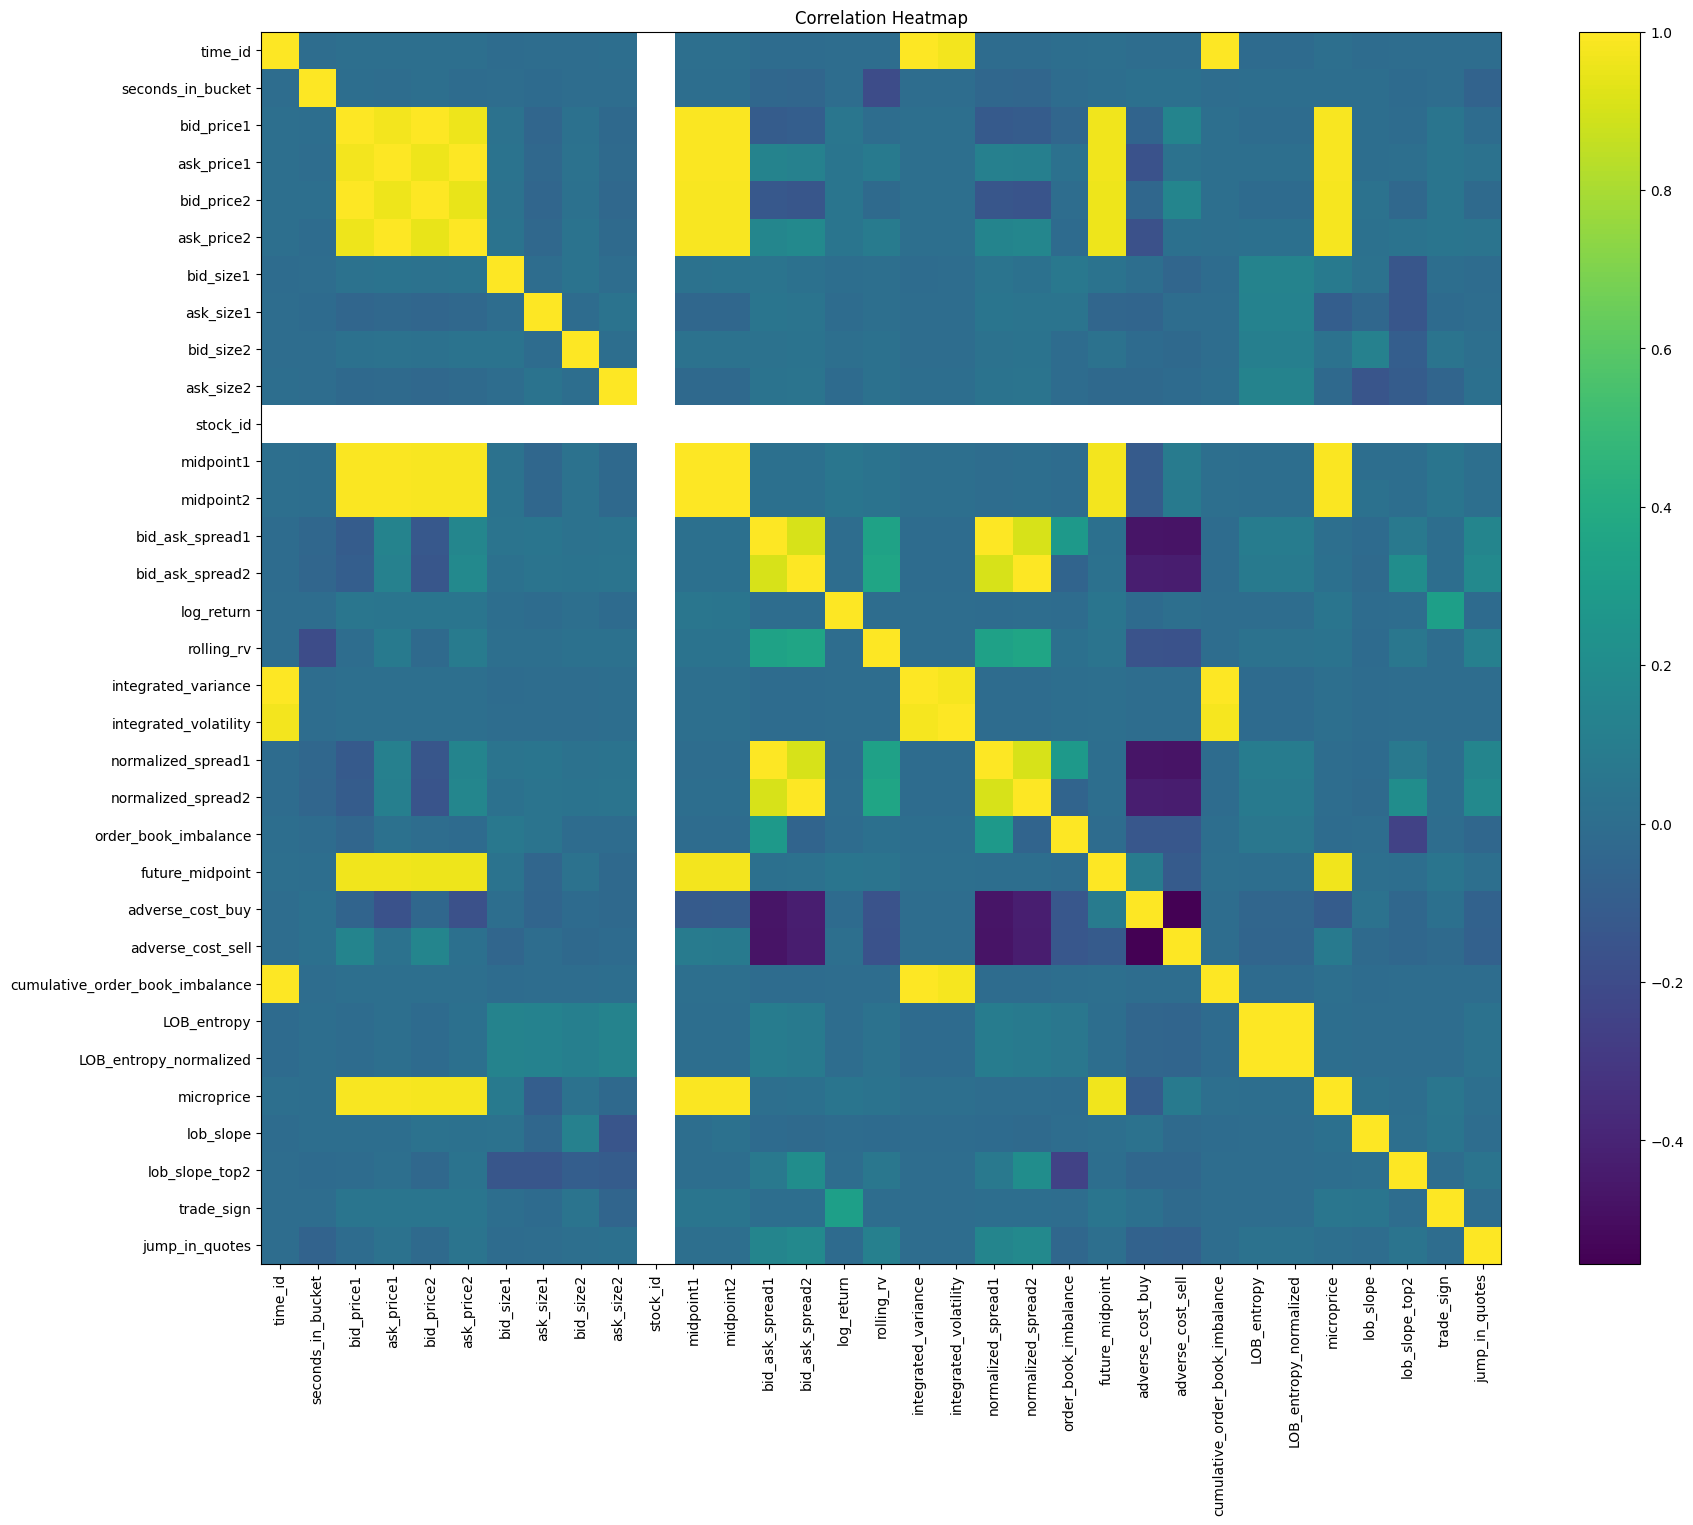
\includegraphics[width=1\textwidth,height=\textheight]{Corr-1.png}

}

\caption{Correlation Plot}

\end{figure}%

\begin{figure}[H]

{\centering 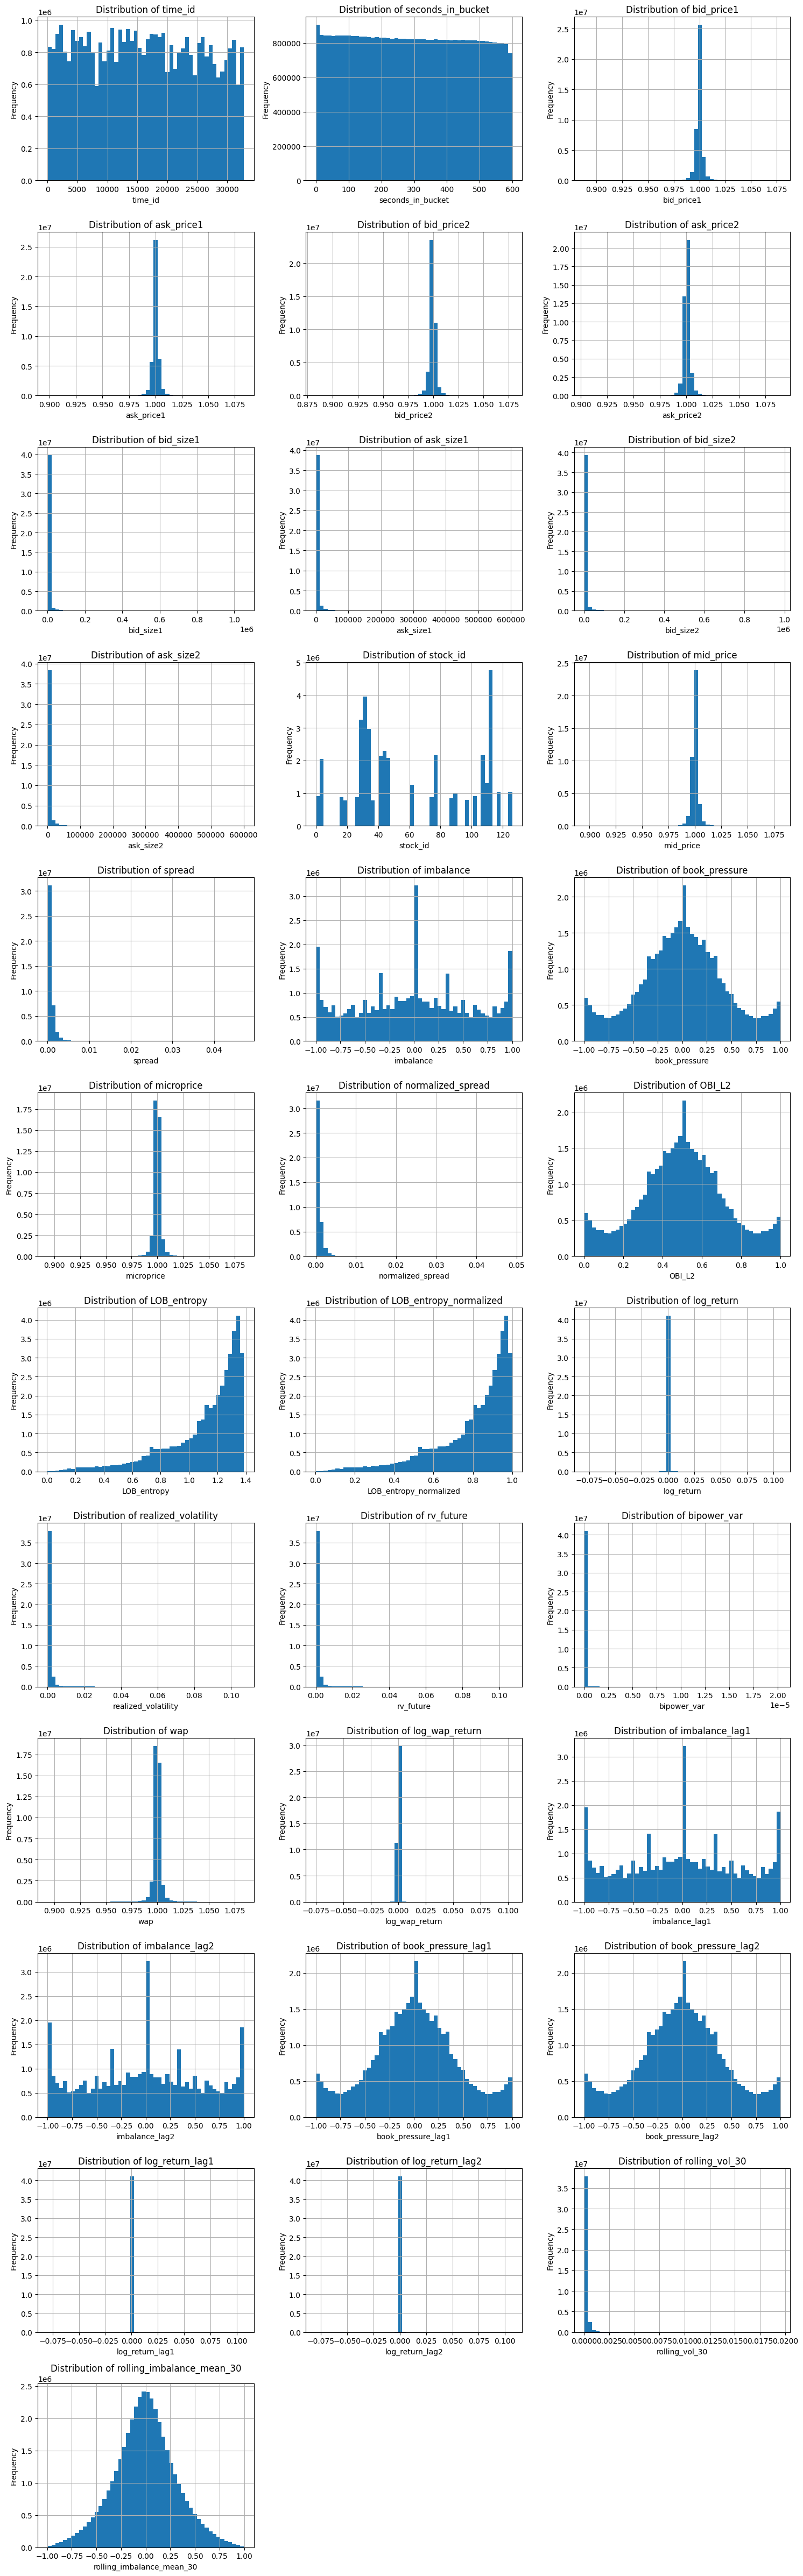
\includegraphics[width=1\textwidth,height=\textheight]{FinalDF-Hist.png}

}

\caption{Data Distribution}

\end{figure}%




\end{document}
